% Created 2021-03-08 man 20:43
% Intended LaTeX compiler: pdflatex
\documentclass[12pt]{article}

%%%% settings when exporting code %%%% 

\usepackage{listings}
\lstdefinestyle{code-small}{
backgroundcolor=\color{white}, % background color for the code block
basicstyle=\ttfamily\small, % font used to display the code
commentstyle=\color[rgb]{0.5,0,0.5}, % color used to display comments in the code
keywordstyle=\color{black}, % color used to highlight certain words in the code
numberstyle=\ttfamily\tiny\color{gray}, % color used to display the line numbers
rulecolor=\color{black}, % color of the frame
stringstyle=\color[rgb]{0,.5,0},  % color used to display strings in the code
breakatwhitespace=false, % sets if automatic breaks should only happen at whitespace
breaklines=true, % sets automatic line breaking
columns=fullflexible,
frame=single, % adds a frame around the code (non,leftline,topline,bottomline,lines,single,shadowbox)
keepspaces=true, % % keeps spaces in text, useful for keeping indentation of code
literate={~}{$\sim$}{1}, % symbol properly display via latex
numbers=none, % where to put the line-numbers; possible values are (none, left, right)
numbersep=10pt, % how far the line-numbers are from the code
showspaces=false,
showstringspaces=false,
stepnumber=1, % the step between two line-numbers. If it's 1, each line will be numbered
tabsize=1,
xleftmargin=0cm,
emph={anova,apply,class,coef,colnames,colNames,colSums,dim,dcast,for,ggplot,head,if,ifelse,is.na,lapply,list.files,library,logLik,melt,plot,require,rowSums,sapply,setcolorder,setkey,str,summary,tapply},
aboveskip = \medskipamount, % define the space above displayed listings.
belowskip = \medskipamount, % define the space above displayed listings.
lineskip = 0pt} % specifies additional space between lines in listings
\lstset{style=code-small}
%%%% packages %%%%%

\usepackage[utf8]{inputenc}
\usepackage[T1]{fontenc}
\usepackage{lmodern}
\usepackage{textcomp}
\usepackage{color}
\usepackage{graphicx}
\usepackage{grffile}
\usepackage{wrapfig}
\usepackage{rotating}
\usepackage{longtable}
\usepackage{multirow}
\usepackage{multicol}
\usepackage{changes}
\usepackage{pdflscape}
\usepackage{geometry}
\usepackage[normalem]{ulem}
\usepackage{amssymb}
\usepackage{amsmath}
\usepackage{amsfonts}
\usepackage{dsfont}
\usepackage{array}
\usepackage{ifthen}
\usepackage{hyperref}
\usepackage{natbib}
\RequirePackage{setspace} % to modify the space between lines - incompatible with footnote in beamer
\renewcommand{\baselinestretch}{1.1}
\geometry{top=1cm}
\usepackage{titlesec}
\usepackage{etoolbox}
\makeatletter
\patchcmd{\ttlh@hang}{\parindent\z@}{\parindent\z@\leavevmode}{}{}
\patchcmd{\ttlh@hang}{\noindent}{}{}{}
\makeatother
\RequirePackage{colortbl} % arrayrulecolor to mix colors
\definecolor{myorange}{rgb}{1,0.2,0}
\definecolor{mypurple}{rgb}{0.7,0,8}
\definecolor{mycyan}{rgb}{0,0.6,0.6}
\newcommand{\lightblue}{blue!50!white}
\newcommand{\darkblue}{blue!80!black}
\newcommand{\darkgreen}{green!50!black}
\newcommand{\darkred}{red!50!black}
\definecolor{gray}{gray}{0.5}
\hypersetup{
citecolor=[rgb]{0,0.5,0},
urlcolor=[rgb]{0,0,0.5},
linkcolor=[rgb]{0,0,0.5},
}
\newenvironment{comment}{\small \color{gray}\fontfamily{lmtt}\selectfont}{\par}
\newenvironment{activity}{\color{orange}\fontfamily{qzc}\selectfont}{\par}
\RequirePackage{pifont}
\RequirePackage{relsize}
\newcommand{\Cross}{{\raisebox{-0.5ex}%
{\relsize{1.5}\ding{56}}}\hspace{1pt} }
\newcommand{\Valid}{{\raisebox{-0.5ex}%
{\relsize{1.5}\ding{52}}}\hspace{1pt} }
\newcommand{\CrossR}{ \textcolor{red}{\Cross} }
\newcommand{\ValidV}{ \textcolor{green}{\Valid} }
\usepackage{stackengine}
\usepackage{scalerel}
\newcommand\Warning[1][3ex]{%
\renewcommand\stacktype{L}%
\scaleto{\stackon[1.3pt]{\color{red}$\triangle$}{\tiny\bfseries !}}{#1}%
\xspace
}
\newcommand\Rlogo{\textbf{\textsf{R}}\xspace} %
\RequirePackage{fancyvrb}
\DefineVerbatimEnvironment{verbatim}{Verbatim}{fontsize=\small,formatcom = {\color[rgb]{0.5,0,0}}}
\lstdefinestyle{code-tiny}{basicstyle=\ttfamily\footnotesize}
\RequirePackage{enumitem} % better than enumerate
\RequirePackage{epstopdf} % to be able to convert .eps to .pdf image files
\RequirePackage{capt-of} %
\RequirePackage{caption} % newlines in graphics
\RequirePackage{tikz-cd} % graph
\RequirePackage{booktabs} % for nice lines in table (e.g. toprule, bottomrule, midrule, cmidrule)
\RequirePackage{amsmath}
\RequirePackage{algorithm}
\RequirePackage[noend]{algpseudocode}
\RequirePackage{dsfont}
\RequirePackage{amsmath,stmaryrd,graphicx}
\RequirePackage{prodint} % product integral symbol (\PRODI)
\usepackage{ifthen}
\usepackage{xifthen}
\usepackage{xargs}
\usepackage{xspace}
\newcommand\defOperator[7]{%
\ifthenelse{\isempty{#2}}{
\ifthenelse{\isempty{#1}}{#7{#3}#4}{#7{#3}#4 \left#5 #1 \right#6}
}{
\ifthenelse{\isempty{#1}}{#7{#3}#4_{#2}}{#7{#3}#4_{#1}\left#5 #2 \right#6}
}
}
\newcommand\defUOperator[5]{%
\ifthenelse{\isempty{#1}}{
#5\left#3 #2 \right#4
}{
\ifthenelse{\isempty{#2}}{\underset{#1}{\operatornamewithlimits{#5}}}{
\underset{#1}{\operatornamewithlimits{#5}}\left#3 #2 \right#4}
}
}
\newcommand{\defBoldVar}[2]{
\ifthenelse{\equal{#2}{T}}{\boldsymbol{#1}}{\mathbf{#1}}
}
\newcommandx\Esp[2][1=,2=]{\defOperator{#1}{#2}{E}{}{\lbrack}{\rbrack}{\mathbb}}
\newcommandx\Prob[2][1=,2=]{\defOperator{#1}{#2}{P}{}{\lbrack}{\rbrack}{\mathbb}}
\newcommandx\Qrob[2][1=,2=]{\defOperator{#1}{#2}{Q}{}{\lbrack}{\rbrack}{\mathbb}}
\newcommandx\Var[2][1=,2=]{\defOperator{#1}{#2}{V}{ar}{\lbrack}{\rbrack}{\mathbb}}
\newcommandx\Cov[2][1=,2=]{\defOperator{#1}{#2}{C}{ov}{\lbrack}{\rbrack}{\mathbb}}
\newcommandx\Binom[2][1=,2=]{\defOperator{#1}{#2}{B}{}{(}{)}{\mathcal}}
\newcommandx\Gaus[2][1=,2=]{\defOperator{#1}{#2}{N}{}{(}{)}{\mathcal}}
\newcommandx\Wishart[2][1=,2=]{\defOperator{#1}{#2}{W}{ishart}{(}{)}{\mathcal}}
\newcommandx\Likelihood[2][1=,2=]{\defOperator{#1}{#2}{L}{}{(}{)}{\mathcal}}
\newcommandx\logLikelihood[2][1=,2=]{\defOperator{#1}{#2}{\ell}{}{(}{)}{}}
\newcommandx\Information[2][1=,2=]{\defOperator{#1}{#2}{I}{}{(}{)}{\mathcal}}
\newcommandx\Score[2][1=,2=]{\defOperator{#1}{#2}{S}{}{(}{)}{\mathcal}}
\newcommandx\Vois[2][1=,2=]{\defOperator{#1}{#2}{V}{}{(}{)}{\mathcal}}
\newcommandx\IF[2][1=,2=]{\defOperator{#1}{#2}{IF}{}{(}{)}{\mathcal}}
\newcommandx\Ind[1][1=]{\defOperator{}{#1}{1}{}{(}{)}{\mathds}}
\newcommandx\Max[2][1=,2=]{\defUOperator{#1}{#2}{(}{)}{min}}
\newcommandx\Min[2][1=,2=]{\defUOperator{#1}{#2}{(}{)}{max}}
\newcommandx\argMax[2][1=,2=]{\defUOperator{#1}{#2}{(}{)}{argmax}}
\newcommandx\argMin[2][1=,2=]{\defUOperator{#1}{#2}{(}{)}{argmin}}
\newcommandx\cvD[2][1=D,2=n \rightarrow \infty]{\xrightarrow[#2]{#1}}
\newcommandx\Hypothesis[2][1=,2=]{
\ifthenelse{\isempty{#1}}{
\mathcal{H}
}{
\ifthenelse{\isempty{#2}}{
\mathcal{H}_{#1}
}{
\mathcal{H}^{(#2)}_{#1}
}
}
}
\newcommandx\dpartial[4][1=,2=,3=,4=\partial]{
\ifthenelse{\isempty{#3}}{
\frac{#4 #1}{#4 #2}
}{
\left.\frac{#4 #1}{#4 #2}\right\rvert_{#3}
}
}
\newcommandx\dTpartial[3][1=,2=,3=]{\dpartial[#1][#2][#3][d]}
\newcommandx\ddpartial[3][1=,2=,3=]{
\ifthenelse{\isempty{#3}}{
\frac{\partial^{2} #1}{\partial #2^2}
}{
\frac{\partial^2 #1}{\partial #2\partial #3}
}
}
\newcommand\Real{\mathbb{R}}
\newcommand\Rational{\mathbb{Q}}
\newcommand\Natural{\mathbb{N}}
\newcommand\trans[1]{{#1}^\intercal}%\newcommand\trans[1]{{\vphantom{#1}}^\top{#1}}
\newcommand{\independent}{\mathrel{\text{\scalebox{1.5}{$\perp\mkern-10mu\perp$}}}}
\newcommand\half{\frac{1}{2}}
\newcommand\normMax[1]{\left|\left|#1\right|\right|_{max}}
\newcommand\normTwo[1]{\left|\left|#1\right|\right|_{2}}
\newcommand\Veta{\boldsymbol{\eta}}
\newcommand\VX{\mathbf{X}}
\author{Brice Ozenne}
\date{\today}
\title{Diagnostics and partial residuals in a linear model}
\hypersetup{
 colorlinks=true,
 pdfauthor={Brice Ozenne},
 pdftitle={Diagnostics and partial residuals in a linear model},
 pdfkeywords={},
 pdfsubject={},
 pdfcreator={Emacs 27.0.50 (Org mode 9.0.4)},
 pdflang={English}
 }
\begin{document}

\maketitle

\section*{Summary}
\label{sec:org15aad81}
In the document we provide a brief introduction of R (sections
\ref{sec:Rsoftware}, \ref{sec:Data}, \ref{sec:descriptive}) and to the linear model
(sections \ref{sec:lm}). We show how some of the underlying hypotheses can
be checked and what to do when there is evidence that one or several
assumptions are not met. We also introduce the notion of partial
residuals (sections \ref{sec:pRes}) and explain how to compute and display
them.

\clearpage

\section{Software}
\label{sec:Rsoftware}
The \Rlogo{} software can be downloaded at
\url{https://cloud.r-project.org/}. R studio provide a convenient user
interface that can be downloaded at
\url{https://www.rstudio.com/products/rstudio/}.  In this document the
\Rlogo{} code will be display in boxes:
\lstset{language=r,label= ,caption= ,captionpos=b,numbers=none}
\begin{lstlisting}
1+1 ## comment about the code
\end{lstlisting}

\begin{verbatim}
[1] 2
\end{verbatim}

while the \Rlogo{} output will be displayed in dark red below the box. 

\bigskip

When starting a fresh \Rlogo{} session, only the core functionalities
of \Rlogo{} are available. Additional functionalities called packages
can be downloaded from the CRAN using the command \texttt{install.packages}:
\lstset{language=r,label= ,caption= ,captionpos=b,numbers=none}
\begin{lstlisting}
install.packages(pkgs = c("lava","car","nlme","ggfortify", "exact2x2",
			  "devtools","reshape2","Publish","officer"))
\end{lstlisting}
Two of the packages we need are not available on CRAN but only on
Github, this is why we also run \footnote{if you do not manage to install
it skip that part, you should still be able to run most of the code
used in this document}:
\lstset{language=r,label= ,caption= ,captionpos=b,numbers=none}
\begin{lstlisting}
devtools::install_github("bozenne/butils")
devtools::install_github("kkholst/gof")
\end{lstlisting}
After having installed the packages, one needs to load them using the
command \texttt{library} to use them in the current \Rlogo{} session:
\lstset{language=r,label= ,caption= ,captionpos=b,numbers=none}
\begin{lstlisting}
library(lava) ## simulate data, latent variable models
library(car) ## miscellaneous sfunction
library(nlme) ## mixed models
library(ggfortify)  ## graphical display
library(butils)  ## miscellaneous function
library(reshape2) ## wide to long format
library(gof)  ## diagnostic tests
library(Publish)  ## table 1
library(officer)  ## export to word
library(exact2x2)  ## compare proportions
\end{lstlisting}

\clearpage

\section{Data}
\label{sec:Data}
\subsection{Generation}
\label{sec:org14a87e9}
\lstset{style=code-tiny}
We will use the dataset generated by the following commands:
\lstset{language=r,label= ,caption= ,captionpos=b,numbers=none}
\begin{lstlisting}
set.seed(10)
m.lvm <- lvm(Y1[100:sigma21]~beta*AgeC+BMI2+Gene,
	     Y2[110:sigma22]~beta*AgeC+BMI2+Gene,
	     Y3[120:sigma23]~beta*AgeC+0.5*BMI2+Gene)
categorical(m.lvm, K = 3) <- ~Gene
distribution(m.lvm, ~Age) <- uniform.lvm(20,50)
distribution(m.lvm, ~BMI) <- gaussian.lvm(mean = 24, sd = 3)
transform(m.lvm, AgeC~Age) <- function(x, ...){x-35}
transform(m.lvm, Id~Age) <- function(x, ...){1:NROW(x)}
transform(m.lvm, BMI2~BMI) <- function(x, ...){(x-24) + (x-24)^2}
latent(m.lvm) <- ~AgeC+BMI2

p1 <- c(beta = 1, sigma21 = 1, sigma22 = 2, sigma23 = 3)
p2 <- c(beta = -1, sigma21 = 4, sigma22 = 4, sigma23 = 4)
d <- rbind(cbind(lava::sim(n = 1e2, m.lvm, latent=FALSE, p = p1), Gender = "Male"),
	   cbind(lava::sim(n = 1e2, m.lvm, latent=FALSE, p = p2), Gender = "Female")
	   )

d$Gender <- as.factor(d$Gender)
d$Gene <- factor(d$Gene, labels = c("A","B","C"))
d$Y1 <- round(d$Y1,1)
d$Y2 <- round(d$Y2,1)
d$Age <- round(d$Age,1)
d$BMI <- round(d$BMI,1)
d <- d[,c("Id","Age","Gender","BMI","Gene","Y1","Y2","Y3")]
head(d)
\end{lstlisting}

\begin{verbatim}
  Id  Age Gender  BMI Gene    Y1    Y2       Y3
1  1 44.2   Male 23.8    A 109.1 120.8 131.7429
2  2 41.3   Male 27.5    B 123.2 133.9 136.3850
3  3 27.4   Male 30.6    A 140.6 154.0 136.1408
4  4 35.3   Male 25.2    C 104.4 116.2 125.0175
5  5 37.1   Male 21.8    A 105.0 113.2 123.6257
6  6 29.9   Male 18.1    C 125.9 136.2 131.7966
\end{verbatim}
\lstset{style=code-small}

We will then export the data in a .csv format using 
\lstset{language=r,label= ,caption= ,captionpos=b,numbers=none}
\begin{lstlisting}
write.csv(d, "data.csv", row.names = FALSE)
\end{lstlisting}

\bigskip

\uline{Note:} in "real life" studies, this step does not exist. Instead an
experiment is performed where some data are collected.


\clearpage


\subsection{Data management}
\label{sec:dataManagement}
\subsubsection{Working directory}
\label{sec:org3e83615}

The working directory is where R, by default, look for files
to import and export data or figures. The current working directory
can be accessed using:
\lstset{language=r,label= ,caption= ,captionpos=b,numbers=none}
\begin{lstlisting}
path <- getwd()
path
\end{lstlisting}

\begin{verbatim}
[1] "/home/brice/Documents/GitHub/bozenne.github.io/doc/2020-09-17-linearModel"
\end{verbatim}

It can be changed using the function \texttt{setwd()}:
\lstset{language=r,label= ,caption= ,captionpos=b,numbers=none}
\begin{lstlisting}
path2 <- "~"
setwd(path2)
\end{lstlisting}

We can check that the working directory has indeed changed calling
again \texttt{getwd()}:
\lstset{language=r,label= ,caption= ,captionpos=b,numbers=none}
\begin{lstlisting}
getwd()
\end{lstlisting}

\begin{verbatim}
[1] "/home/brice"
\end{verbatim}

We move back to the original working directory doing:
\lstset{language=r,label= ,caption= ,captionpos=b,numbers=none}
\begin{lstlisting}
setwd(path)
\end{lstlisting}

\subsubsection{Importing the data}
\label{sec:org1c85bb4}

It is a good idea to start by checking that the working directory
contains the data we want to import. For instance the file \texttt{data.csv}
is storing the data, we can use:
\lstset{language=r,label= ,caption= ,captionpos=b,numbers=none}
\begin{lstlisting}
file.exists("data.csv")
\end{lstlisting}

\begin{verbatim}
[1] TRUE
\end{verbatim}

We can also list all files in the current directory with a \texttt{.csv} extension using:
\lstset{language=r,label= ,caption= ,captionpos=b,numbers=none}
\begin{lstlisting}
list.files(pattern = ".csv")
\end{lstlisting}

\begin{verbatim}
[1] "data.csv"
\end{verbatim}

\clearpage

We can also display the first lines of the file using:
\lstset{language=r,label= ,caption= ,captionpos=b,numbers=none}
\begin{lstlisting}
readLines("data.csv")[1:3]
\end{lstlisting}

\begin{verbatim}
[1] "\"Id\",\"Age\",\"Gender\",\"BMI\",\"Gene\",\"Y1\",\"Y2\",\"Y3\""
[2] "1,44.2,\"Male\",23.8,\"A\",109.1,120.8,131.742898261202"        
[3] "2,41.3,\"Male\",27.5,\"B\",123.2,133.9,136.385038040154"
\end{verbatim}

We can see that the columns are separated with \texttt{,} and that the \texttt{.}
indicates the decimal values. Moreover the words such as the columns
names or the subject identities are surrounded by \texttt{\textbackslash{}"} (e.g. \texttt{\textbackslash{}"Id\textbackslash{}"}
stand for Id). Finally in this example there is no missing values but
if there was it is important to know how they are encoded.

\bigskip

 The command to import the data depends on the type of file. Here for
a \texttt{.csv} file we use \texttt{read.csv}. Luckily the default arguments \texttt{sep},
\texttt{dec}, \texttt{quote} are correctly specified:
\lstset{language=r,label= ,caption= ,captionpos=b,numbers=none}
\begin{lstlisting}
args(read.csv)
\end{lstlisting}

\begin{verbatim}
function (file, header = TRUE, sep = ",", quote = "\"", dec = ".", 
    fill = TRUE, comment.char = "", ...) 
NULL
\end{verbatim}

The argument \texttt{header} set to \texttt{TRUE} indicates that the first line of
the dataset contains the column names (and not the actual data). The
\texttt{...} indicates there are additional arguments that are not shown here
(see the documentation using \texttt{help(read.csv)}). For instance, in
presence of missing values, one would need to specify the argument
\texttt{na.string}. Here it is sufficient to do:
\lstset{language=r,label= ,caption= ,captionpos=b,numbers=none}
\begin{lstlisting}
dfW <- read.csv("data.csv")
\end{lstlisting}

Other functions exists to import other types of data,
e.g. \texttt{read.table} for \texttt{.txt} files, \texttt{read.xlsx} from the xlsx package
for \texttt{.xlsx} file, or \texttt{read.spss} from the foreign package for spss
data files. One should always inspect if R has correctly imported the
data, e.g. using:
\lstset{language=r,label= ,caption= ,captionpos=b,numbers=none}
\begin{lstlisting}
str(dfW)
\end{lstlisting}

\begin{verbatim}
'data.frame':	200 obs. of  8 variables:
 $ Id    : int  1 2 3 4 5 6 7 8 9 10 ...
 $ Age   : num  44.2 41.3 27.4 35.3 37.1 29.9 33.1 26 43.6 43.5 ...
 $ Gender: Factor w/ 2 levels "Female","Male": 2 2 2 2 2 2 2 2 2 2 ...
 $ BMI   : num  23.8 27.5 30.6 25.2 21.8 18.1 18.1 21.2 27.6 22.1 ...
 $ Gene  : Factor w/ 3 levels "A","B","C": 1 2 1 3 1 3 3 1 3 3 ...
 $ Y1    : num  109 123 141 104 105 ...
 $ Y2    : num  121 134 154 116 113 ...
 $ Y3    : num  132 136 136 125 124 ...
\end{verbatim}

In this example, the two columns contain character strings (\texttt{Factor}
is a type of character strings in R) and the rest contains numerical
values.

\subsubsection{Data processing}
\label{sec:org0d6d058}

Often the raw data needs to be transformed before being analyzed:
\begin{itemize}
\item A typical example is when one need to deal with the variable:
\end{itemize}
\lstset{language=r,label= ,caption= ,captionpos=b,numbers=none}
\begin{lstlisting}
gender <- c(1,0,1,0,1) ## what is 1? what is 0?
\end{lstlisting}

This is already better:
\lstset{language=r,label= ,caption= ,captionpos=b,numbers=none}
\begin{lstlisting}
female <- c(1,0,1,0,1) ## we can guess that 1: female and 0: male
\end{lstlisting}

but it is a good practice in such situation to rename the actual
values into something understandable:
\lstset{language=r,label= ,caption= ,captionpos=b,numbers=none}
\begin{lstlisting}
factor(gender, levels = 0:1, labels = c("Female","Male"))
\end{lstlisting}

\begin{verbatim}
[1] Male   Female Male   Female Male  
Levels: Female Male
\end{verbatim}

\begin{itemize}
\item With repeated measurements per individual, one often needs to
reshape his dataset from the wide format (one line per individual)
to the long format (one line per measurement). This can be done
using the \texttt{melt} method. The opposite operation can be performed
using \texttt{dcast}.
\end{itemize}

\lstset{language=r,label= ,caption= ,captionpos=b,numbers=none}
\begin{lstlisting}
str(dfW)
\end{lstlisting}

\begin{verbatim}
'data.frame':	200 obs. of  8 variables:
 $ Id    : int  1 2 3 4 5 6 7 8 9 10 ...
 $ Age   : num  44.2 41.3 27.4 35.3 37.1 29.9 33.1 26 43.6 43.5 ...
 $ Gender: Factor w/ 2 levels "Female","Male": 2 2 2 2 2 2 2 2 2 2 ...
 $ BMI   : num  23.8 27.5 30.6 25.2 21.8 18.1 18.1 21.2 27.6 22.1 ...
 $ Gene  : Factor w/ 3 levels "A","B","C": 1 2 1 3 1 3 3 1 3 3 ...
 $ Y1    : num  109 123 141 104 105 ...
 $ Y2    : num  121 134 154 116 113 ...
 $ Y3    : num  132 136 136 125 124 ...
\end{verbatim}

\lstset{language=r,label= ,caption= ,captionpos=b,numbers=none}
\begin{lstlisting}
dfL <- reshape2::melt(dfW, id.vars = c("Id","Gender","Age","BMI","Gene"),
		      measure.vars = c("Y1","Y2","Y3"),
		      value.name = "score",variable.name = "outcome")
head(dfL)
\end{lstlisting}

\begin{verbatim}
  Id Gender  Age  BMI Gene outcome score
1  1   Male 44.2 23.8    A      Y1 109.1
2  2   Male 41.3 27.5    B      Y1 123.2
3  3   Male 27.4 30.6    A      Y1 140.6
4  4   Male 35.3 25.2    C      Y1 104.4
5  5   Male 37.1 21.8    A      Y1 105.0
6  6   Male 29.9 18.1    C      Y1 125.9
\end{verbatim}


\begin{itemize}
\item It is often a good idea to restrict the dataset to the relevant
variables (e.g. remove genetic data if they are not of interest). It
is easier to work with and to display in the next steps. This can
for instance be done by defining the variables of interest:
\end{itemize}
\lstset{language=r,label= ,caption= ,captionpos=b,numbers=none}
\begin{lstlisting}
keep.var <- c("Id","BMI","Y1")
\end{lstlisting}

We can check that the variables defined in \texttt{keep.var} are in \texttt{df}:
\lstset{language=r,label= ,caption= ,captionpos=b,numbers=none}
\begin{lstlisting}
keep.var %in% names(dfW)
\end{lstlisting}

\begin{verbatim}
[1] TRUE TRUE TRUE
\end{verbatim}

and then subset the initial dataset:
\lstset{language=r,label= ,caption= ,captionpos=b,numbers=none}
\begin{lstlisting}
dfW.red <- dfW[,keep.var]
head(dfW.red)
\end{lstlisting}

\begin{verbatim}
  Id  BMI    Y1
1  1 23.8 109.1
2  2 27.5 123.2
3  3 30.6 140.6
4  4 25.2 104.4
5  5 21.8 105.0
6  6 18.1 125.9
\end{verbatim}

\begin{itemize}
\item Often after having imported the data we want to change its column
names. First we need to know the current column names. The \texttt{names}
function can be used to output all the column names:
\end{itemize}
\lstset{language=r,label= ,caption= ,captionpos=b,numbers=none}
\begin{lstlisting}
names(dfW)
\end{lstlisting}

\begin{verbatim}
[1] "Id"     "Age"    "Gender" "BMI"    "Gene"   "Y1"     "Y2"     "Y3"
\end{verbatim}

Alternatively the \texttt{grep} function will output any column name
containing a given string of characters:
\lstset{language=r,label= ,caption= ,captionpos=b,numbers=none}
\begin{lstlisting}
grep(pattern = "Y", x = names(dfW), value = TRUE)
\end{lstlisting}

\begin{verbatim}
[1] "Y1" "Y2" "Y3"
\end{verbatim}

Then, we can rename columns one at a time using:
\lstset{language=r,label= ,caption= ,captionpos=b,numbers=none}
\begin{lstlisting}
names(dfW)[names(dfW) == "Y1"] <- "baseline_score"
names(dfW)[names(dfW) == "Y2"] <- "followup_score"
names(dfW)[names(dfW) == "Y3"] <- "final_score"
head(dfW)
\end{lstlisting}

\begin{verbatim}
  Id  Age Gender  BMI Gene baseline_score followup_score final_score
1  1 44.2   Male 23.8    A          109.1          120.8    131.7429
2  2 41.3   Male 27.5    B          123.2          133.9    136.3850
3  3 27.4   Male 30.6    A          140.6          154.0    136.1408
4  4 35.3   Male 25.2    C          104.4          116.2    125.0175
5  5 37.1   Male 21.8    A          105.0          113.2    123.6257
6  6 29.9   Male 18.1    C          125.9          136.2    131.7966
\end{verbatim}

To rename several columns at the same time we can use:
\lstset{language=r,label= ,caption= ,captionpos=b,numbers=none}
\begin{lstlisting}
old2new <- c("baseline_score" = "Y1", 
	     "followup_score" = "Y2",
	     "final_score" = "Y3")
names(dfW)[match(names(old2new),names(dfW))] <- old2new
head(dfW)
\end{lstlisting}

\begin{verbatim}
  Id  Age Gender  BMI Gene    Y1    Y2       Y3
1  1 44.2   Male 23.8    A 109.1 120.8 131.7429
2  2 41.3   Male 27.5    B 123.2 133.9 136.3850
3  3 27.4   Male 30.6    A 140.6 154.0 136.1408
4  4 35.3   Male 25.2    C 104.4 116.2 125.0175
5  5 37.1   Male 21.8    A 105.0 113.2 123.6257
6  6 29.9   Male 18.1    C 125.9 136.2 131.7966
\end{verbatim}

Other useful functions are \texttt{tolower} to convert characters to lower
case and \texttt{gsub} to remove a specific pattern in a character vector, e.g.:
\lstset{language=r,label= ,caption= ,captionpos=b,numbers=none}
\begin{lstlisting}
gsub(pattern = ".", replacement = "", x = c("a..","b..."), fixed = TRUE)
\end{lstlisting}

\begin{verbatim}
[1] "a" "b"
\end{verbatim}

Many of the other data processing steps are specific to each study and
we won't discuss them in this document. 


\section{Descriptive statistics}
\label{sec:descriptive}
Before doing any analysis, it is a good practice to describe the data
that are to be analyzed. The has several aims:
\begin{itemize}
\item \textbf{check that that database contains the population of interest},
i.e. individuals in the database are indeed those the we want to
study and we have all of them.
\item \textbf{check that the collected values are plausible}, e.g. if the inclusion
criteria include that the age range is between 18 and 99 years, then
one should check that this is indeed the case.
\item \textbf{check that the collected values are coded as expected}, e.g. age is
usually coded in years (and not in months).
\item \textbf{check that the collected values are distributed as expected},
e.g. is there missing values? Are the values uniformly spread?
Bimodal? Concentrated at low or high values?
\end{itemize}

Note: one should checks that for all the variables of interest. This
can appear time-consuming but can really save you time at latter
stages. 

\begin{itemize}
\item \textbf{produce your table 1} i.e. a descriptive table of your cohort that
is almost always included in an article. You can for instance use
the function \texttt{univariateTable} from the Publish package:
\end{itemize}
\lstset{language=r,label= ,caption= ,captionpos=b,numbers=none}
\begin{lstlisting}
myTable1 <- univariateTable(Gender ~ Age + BMI + Y1 + Y2 + Y3, 
			    data = dfW)
myTable1
\end{lstlisting}

\begin{verbatim}
  Variable     Level Female (n=100) Male (n=100) Total (n=200) p-value
1      Age mean (sd)     33.9 (8.7)     35.1 (9)    34.5 (8.9)  0.3459
2      BMI mean (sd)     24.2 (2.6)   23.8 (3.4)        24 (3)  0.4307
3       Y1 mean (sd)   109.1 (13.8)   112.2 (17)  110.7 (15.5)  0.1606
4       Y2 mean (sd)   119.1 (13.3)   122.4 (17)  120.7 (15.4)  0.1335
5       Y3 mean (sd)   126.1 (10.7)   127 (11.5)  126.6 (11.1)  0.5601
\end{verbatim}

You can also export this table in a word document with the package
officer:
\lstset{language=r,label= ,caption= ,captionpos=b,numbers=none}
\begin{lstlisting}
myTable1.doc <- body_add_table(x = read_docx(), 
			       value =  summary(myTable1)) 
print(myTable1.doc, target = "./Table1.docx")
\end{lstlisting}

To keep the code simple, we only present here a very basic application
of these tools. More complex tables with a nicer display in word can
be obtain with a bit of coding.

\clearpage

\begin{itemize}
\item \textbf{make synthetic representations of your data} using graphs or
images. This can be useful to visualize your data and help your
collaborators to understand what you have collected or what you are
trying to show.
\end{itemize}

\lstset{language=r,label= ,caption= ,captionpos=b,numbers=none}
\begin{lstlisting}
library(ggplot2)
gg <- ggplot(dfL, aes(x = BMI, y = score, color = Gender, group = Gender))
gg <- gg + geom_point()
gg <- gg + facet_wrap(~outcome, labeller = label_both)
gg <- gg + geom_smooth(method = "lm", se = FALSE)
gg
\end{lstlisting}

\begin{verbatim}
`geom_smooth()` using formula 'y ~ x'
\end{verbatim}

\begin{center}
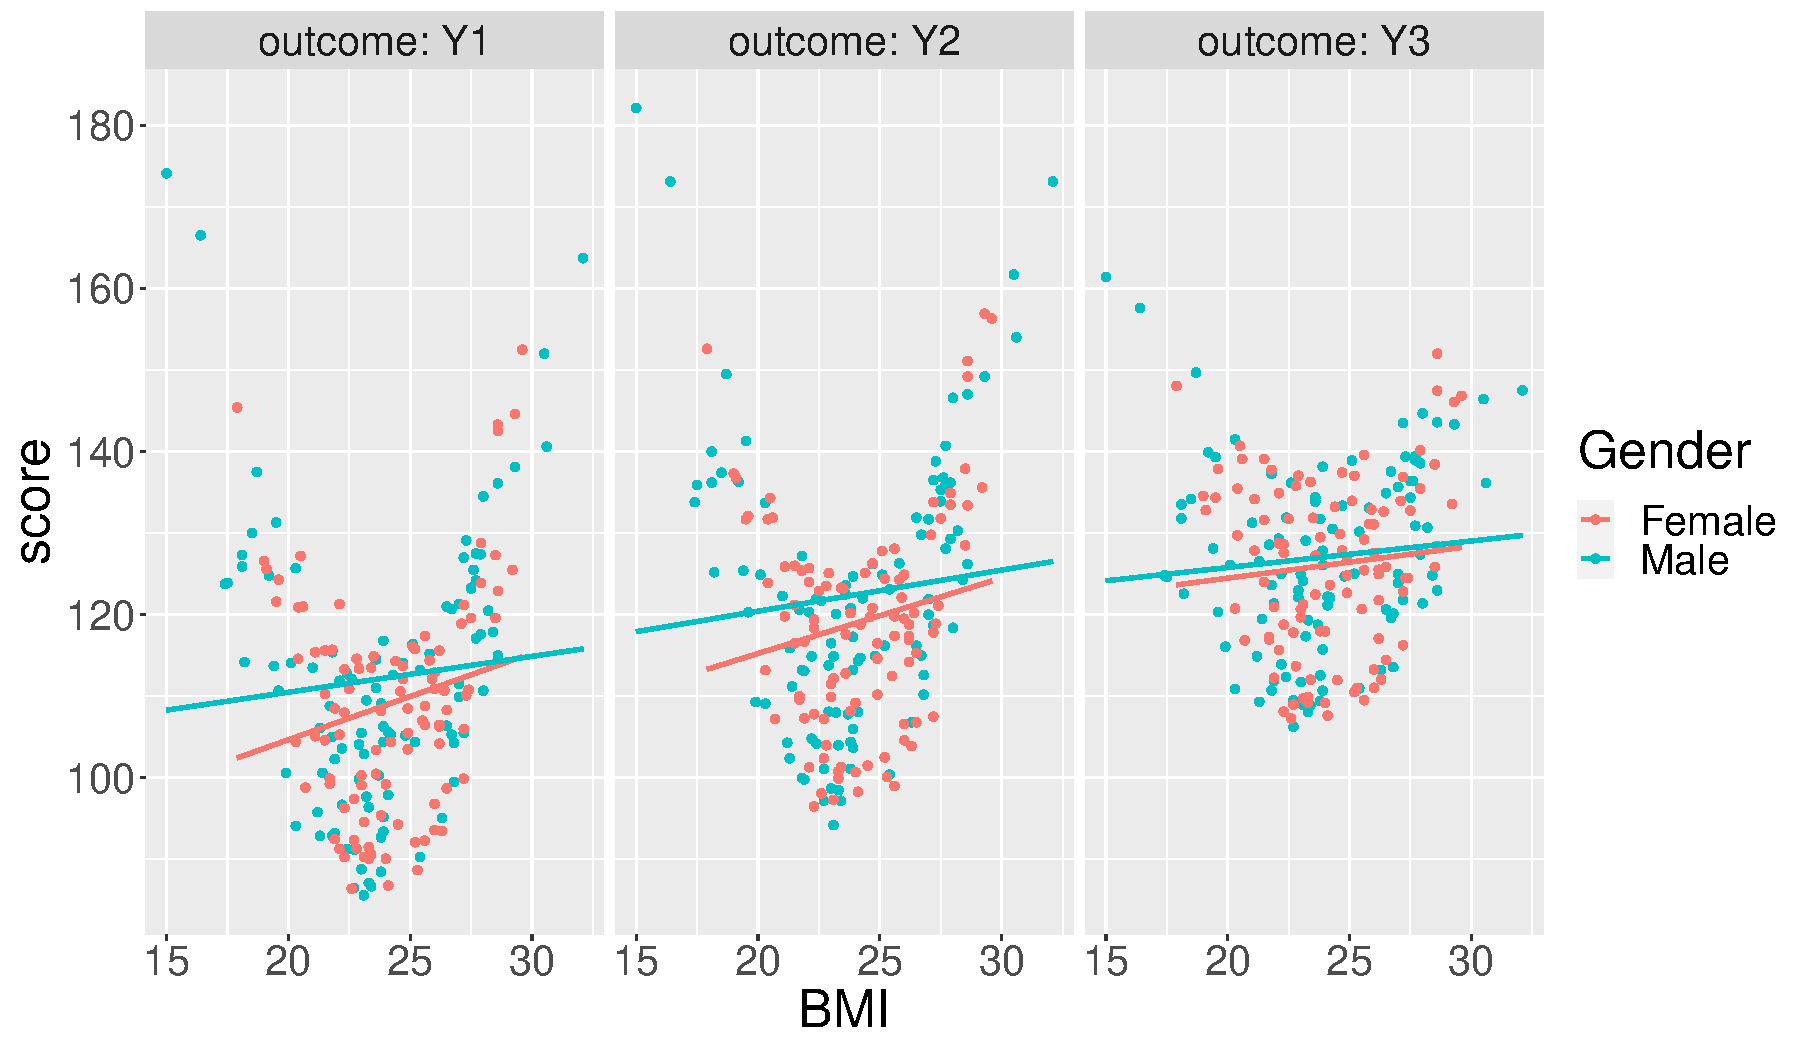
\includegraphics[width=.9\linewidth]{./figures/descriptive.pdf}
\end{center}

You can then export the figure in a folder \texttt{figures} using:
\lstset{language=r,label= ,caption= ,captionpos=b,numbers=none}
\begin{lstlisting}
pdf("./figures/descriptive.pdf", width = 12)
gg + theme(text = element_text(size=25))
dev.off()
\end{lstlisting}

\begin{itemize}
\item \textbf{Compare percentages when considering categorical data}: the usual
way to compare the distribution of a categorical variable between
two groups is to run a Fisher test using \texttt{fisher.test} in the R
software. It returns a p-value and an estimate of the odd ratio with
its confidence interval. For instance, consider the following
dataset:
\end{itemize}
\lstset{language=r,label= ,caption= ,captionpos=b,numbers=none}
\begin{lstlisting}
mytable <- rbind(c(8,5), c(4,15))
dimnames(mytable) <- list(c("control","treatment"), c("-","+"))
mytable
\end{lstlisting}

\begin{verbatim}
          -  +
control   8  5
treatment 4 15
\end{verbatim}
The Fisher test outputs:
\lstset{language=r,label= ,caption= ,captionpos=b,numbers=none}
\begin{lstlisting}
fisher.test(mytable)
\end{lstlisting}

\begin{verbatim}
	Fisher's Exact Test for Count Data

data:  mytable
p-value = 0.02996
alternative hypothesis: true odds ratio is not equal to 1
95 percent confidence interval:
  0.9953576 38.7853302
sample estimates:
odds ratio 
  5.622612
\end{verbatim}

This approach admits two drawbacks:
\begin{itemize}
\item the p-value may not agree with the confidence interval of the odd
ratio regarding the rejection of the null hypothesis
\item the odd ratio is a rather complex quantity to understand.
\end{itemize}
Instead one can use the function \texttt{binomMeld.test} (package \emph{exact2x2})
to perform a test on the proportions:
\lstset{language=r,label= ,caption= ,captionpos=b,numbers=none}
\begin{lstlisting}
binomMeld.test(x1=mytable["control","+"],n1=sum(mytable["control",]),
	       x2=mytable["treatment","+"],n2=sum(mytable["treatment",]),
	       parmtype="difference")
\end{lstlisting}

\begin{verbatim}
	melded binomial test for difference

data:  sample 1:(5/13), sample 2:(15/19)
proportion 1 = 0.38462, proportion 2 = 0.78947, p-value = 0.05077
alternative hypothesis: true difference is not equal to 0
95 percent confidence interval:
 -0.001077177  0.715576028
sample estimates:
difference (p2-p1) 
         0.4048583
\end{verbatim}

This time the p-value is consistent with the confidence interval. 
\clearpage


\section{Introduction to the linear model}
\label{sec:lm}
Imagine we would like to model the age effect on the outcome, but
accounting for a possible gender and gene effect. In \Rlogo{} we would
use the \texttt{lm} function:
\lstset{language=r,label= ,caption= ,captionpos=b,numbers=none}
\begin{lstlisting}
e.lm <- lm(Y1 ~ Gender + Age + Gene + BMI, data = dfW)
e.lm
\end{lstlisting}

\begin{verbatim}

Call:
lm(formula = Y1 ~ Gender + Age + Gene + BMI, data = dfW)

Coefficients:
(Intercept)   GenderMale          Age        GeneB        GeneC          BMI  
    91.5610       3.7984      -0.1358       7.8329       5.8120       0.7365
\end{verbatim}

Denote for the \(i-th\) patient its outcome value by \(Y_i\) (can be
any real number), its gender value by \(Gender_i\) (can be "Male" or
"Female"), its gene value by \(Gene_i\) (can be "A", "B", or
"C"), and its BMI value by \(BMI_i\). Mathematically, this linear model can be written:
\begin{align*}
Y_i =& \alpha + \beta_{Gender} * \Ind[Gender_i="Male"] + \beta_{Age} * Age_i + \beta_{GeneB} *  \Ind[Gene_i="B"] + \beta_{GeneC} * \Ind[Gene_i="C"] \\
& + \beta_{BMI} * BMI_i + \varepsilon_i
\end{align*}
where \(\boldsymbol{\beta} =
(\alpha,\beta_{Gender},\beta_{Age},\beta_{GeneB},\beta_{GeneC},\beta_{BMI})\) is
the vector of model parameters. Their value is shown just above
(e.g. \(\alpha=21.3988\)). Here \(\Ind[.]\) denotes the indicator
function taking value 1 if "." is true and 0
otherwise. \(\varepsilon_i\) is the residual error, i.e. the
difference between the observed value and the fitted value. Consider
for instance the first individual:
\lstset{language=r,label= ,caption= ,captionpos=b,numbers=none}
\begin{lstlisting}
d[1,]
\end{lstlisting}

\begin{verbatim}
  Id  Age Gender  BMI Gene    Y1    Y2       Y3
1  1 44.2   Male 23.8    A 109.1 120.8 131.7429
\end{verbatim}
its observed value is 109.2 and we can computed its fitted value as:
\begin{align*}
\hat{Y}_1 &= \widehat{\alpha} + \widehat{\beta}_{Gender} * 0 + \widehat{\beta}_{Age} 48 + \widehat{\beta}_{GeneB} * 0 + \widehat{\beta}_{GeneC} * 0 \\
          &= 91.5610 + 3.7984 * 1 - 0.1358 * 44.2 + 7.8329 * 0 + 5.8120 * 0 + 0.7365 * 23.8 \\
          & = 106.8857
\end{align*}

Here the hat on top of the \(\beta\) refer to the estimated coefficient.

\clearpage 

This can also be obtained using the \texttt{fitted} method in \Rlogo{} (the
discrepancy comes from rounding the coefficient values at the 4th
digit):
\lstset{language=r,label= ,caption= ,captionpos=b,numbers=none}
\begin{lstlisting}
fitted(e.lm)[1]
\end{lstlisting}

\begin{verbatim}
       1 
106.8839
\end{verbatim}

Often, for conciseness, this linear model can be abbreviated as:
\begin{align*}
Y_i = X_i \boldsymbol{\beta} + \varepsilon_i
\end{align*}
where \(X_i = \left(1, \Ind[Gender_i="Male"], Age_i,
\Ind[Gene_i="B"], \Ind[Gene_i="C"]\right)\) and \(X_i
\boldsymbol{\beta}\) is the matrix product between the row vector
\(X_i\) and the column vector \(\boldsymbol{\beta}\). More generally,
i.e. at the population level instead of the individual level, we also
write \(Y = X \boldsymbol{\beta} + \varepsilon\) to describe the
relationship between the random variables \(Y\), \(X\),
\(\varepsilon\).

\subsection{Assumptions}
\label{sec:orgfb1c5eb}
A linear model \(Y = X \beta + \varepsilon\) is a model studying the
 effects (\(\beta\)) of covariates (\(X\)) on the expected value of
 the outcome \(Y\). Maximum likelihood (ML) estimation leads to
 unbiased estimates of \(\beta\) if the following assumptions are
 satisfied:
\begin{itemize}
\item \textbf{(A0)}: no unobserved confounders.
\item \textbf{(A1)}: \(\Esp[Y_i|X] = X_i \beta\) correct specification of the
functional form of the covariates.
\item \textbf{(A2)}: identically distributed and \textbf{(A3)} independent
residuals. \newline Under the normality assumption, it simplifies to
\textbf{(A2)} homoschedasticity \(\Var[Y_i|X]= \sigma^2\) and \textbf{(A3)}
uncorrelatedness \(\forall i \neq j\), \(\Cov[Y_i,Y_j|X]= 0\).
\end{itemize}
While not needed per se, the assumption of:
\begin{itemize}
\item \textbf{(A4)}: normally distributed residuals is often mentioned since (i)
normality of the estimates holds exactly in finite samples (instead
of asymptotically) i.e. p-values/CIs are reliable even in small
samples, (ii) it ensures that MLE is the best estimation procedure,
(iii) checking \textbf{(A2)} and \textbf{(A3)} is simplified.
\end{itemize}
Additional assumptions (automatically fullfield under normality) are
typically necessary to ensure reliable and interpretable estimates:
\begin{itemize}
\item \textbf{(A4-bis)}: approximately symmetric and unimodal - otherwise modeling the
expected value (aka the mean value) may not be very relevant.
\item \textbf{(A5)}: absence of outliers - otherwise the estimates may be very
sensitive to the value of a few observations which is often
undesirable.
\end{itemize}

\clearpage

\subsection{Interpretation of the regression coefficients}
\label{sec:interpretationLM}
If the assumptions (A1-A3), \(\beta_{age}\) reflect the association
between age and the outcome. This means that for fixed gene, gender,
and BMI, if we observe an individual A one year older than an
individual B then we would also expect that its value for the outcome
\(Y\) to differ by \(\beta_{age}\). \newline If we in addition make causal
assumptions (mainly A0: no unobserved confounder) then we can
interpret \(\beta_{Age}\) as the effect of age on the outcome. This
means that if we could change the age of an individual by one unit
then its variation in outcome should be \(\beta_{age}\).


\subsection{Hypothesis testing}
\label{sec:orgd700c45}

We want to formally test whether there is an effect of age on the
outcome. We first need to make the distinction between:
\begin{itemize}
\item \(\beta^0_{age}\) the true but unknown age effect (may be 1.5)
\item \(\widehat{\beta}_{age}\) the estimated age effect (here 1.5326 using maximum likelihood)
\end{itemize}
We would like to test the null hypothesis of no age effect:
\begin{align*}
(\Hypothesis[0]) \; \beta^0_{age} = 0
\end{align*}
 Since the parameters are estimated by ML and assuming that the model
is correctly specified, we know that the asymptotic distribution of
the parameter is Gaussian. This means that for large sample size, the
fluctuation of the estimated values follows a normal distribution. For
instance:
\begin{align*}
\hat{\beta}_{age} \underset{n \rightarrow \infty}{\sim} \Gaus[\beta^0_{age},\sigma^2_{\beta_{age}}]
\end{align*}
where \(\sigma^2_{\beta_{age}}\) is the variance of the MLE, i.e. the
uncertainty surrounding our estimation of the association. It follows that:
\begin{align}
t_{\beta_{age}} = \frac{\hat{\beta}_{age}-\beta^0_{age}}{\sigma^2_{\beta_{age}}} \underset{n \rightarrow \infty}{\sim} \Gaus[0,1] \label{eq:uniWald}
\end{align}
So under the null hypothesis of no association between the outcome and
the exposure the statistic \(t_{\beta_{age}}\) should follow a standard
normal distribution. Very low or very large values are unlikely to be
observed and would indicate that the null hypothesis does not
hold. This is called a (univariate) Wald test. 

\clearpage 

The result of this tests can be obtained using the \texttt{summary}
method \footnote{In reality R is automatically performing a correction that
improves the control of the type 1 error. Indeed we usually don't know
\(\sigma^2_{\beta_{age}}\) and plugging-in its estimate in equation
\eqref{eq:uniWald} modifies the distribution of \(t_{\beta_{age}}\) in
small samples. The correction uses a Student's t distribution instead
of a Gaussian distribution.}:
\lstset{language=r,label= ,caption= ,captionpos=b,numbers=none}
\begin{lstlisting}
summary(e.lm)$coef
\end{lstlisting}

\begin{verbatim}
              Estimate Std. Error   t value     Pr(>|t|)
(Intercept) 91.5609817  9.4890315  9.649139 3.049271e-18
GenderMale   3.7984283  2.1504309  1.766357 7.890869e-02
Age         -0.1358252  0.1222051 -1.111452 2.677492e-01
GeneB        7.8328783  2.6882498  2.913746 3.990606e-03
GeneC        5.8120279  2.5395657  2.288591 2.318060e-02
BMI          0.7364696  0.3583963  2.054903 4.122862e-02
\end{verbatim}

95\% confidence intervals for the model parameters can then be obtained
using the \texttt{confint} method:
\lstset{language=r,label= ,caption= ,captionpos=b,numbers=none}
\begin{lstlisting}
confint(e.lm)
\end{lstlisting}

\begin{verbatim}
                  2.5 %     97.5 %
(Intercept) 72.84607298 110.275890
GenderMale  -0.44279672   8.039653
Age         -0.37684645   0.105196
GeneB        2.53093057  13.134826
GeneC        0.80332490  10.820731
BMI          0.02961616   1.443323
\end{verbatim}

Note that based on the estimate and standard errors, we could compute
the p-value ourself:
\lstset{language=r,label= ,caption= ,captionpos=b,numbers=none}
\begin{lstlisting}
beta <- summary(e.lm)$coef[,"Estimate"]
sigma <- summary(e.lm)$coef[,"Std. Error"]
df <- df.residual(e.lm)
t.abs <- abs(beta/sigma)
rbind(asymptotic = 2*(1-pnorm(t.abs)),
      corrected = 2*(1-pt(t.abs, df = df)))
cat("degrees of freedom:", df,"\n")
\end{lstlisting}

\begin{verbatim}
           (Intercept) GenderMale       Age       GeneB      GeneC        BMI
asymptotic           0 0.07733600 0.2663737 0.003571198 0.02210311 0.03988840
corrected            0 0.07890869 0.2677492 0.003990606 0.02318060 0.04122862
degrees of freedom: 194
\end{verbatim}

\clearpage 
and the confidence intervals:
\lstset{language=r,label= ,caption= ,captionpos=b,numbers=none}
\begin{lstlisting}
cbind(normLower = beta + qnorm(0.025) * sigma, 
      normUpper = beta + qnorm(0.975) * sigma,
      tLower = beta + qt(0.025, df = df) * sigma, 
      tUpper = beta + qt(0.975, df = df) * sigma)
\end{lstlisting}

\begin{verbatim}
              normLower   normUpper      tLower     tUpper
(Intercept) 72.96282173 110.1591416 72.84607298 110.275890
GenderMale  -0.41633879   8.0131954 -0.44279672   8.039653
Age         -0.37534289   0.1036925 -0.37684645   0.105196
GeneB        2.56400558  13.1017511  2.53093057  13.134826
GeneC        0.83457057  10.7894853  0.80332490  10.820731
BMI          0.03402571   1.4389134  0.02961616   1.443323
\end{verbatim}

\subsection{Checking assumptions made when fitting a linear model}
\label{sec:org8ea3ceb}

\subsubsection{\textbf{(A0)}: no unobserved confounders}
\label{sec:org952d969}
\textbf{(A0)} is in general impossible to check.

\subsubsection{\textbf{(A1)}: correct specification of the functional}
\label{sec:org4634a94}
\textbf{(A1)} can be (artificially) decomposed into two part:
\begin{itemize}
\item in absence of interaction, \textbf{is the effect of the continuous
variables correctly modeled?} Typically it is modeled as a linear
effect and the question is is there a non-linear effect. We can look
at the plot of the covariate vs. the residuals and search for any
trend:
\end{itemize}
\lstset{language=r,label= ,caption= ,captionpos=b,numbers=none}
\begin{lstlisting}
gg <- ggplot(d, aes(x = BMI, y = residuals(e.lm)))
gg <- gg + geom_point() + geom_smooth() + ylab("residuals")
gg
\end{lstlisting}

\begin{verbatim}
`geom_smooth()` using method = 'loess' and formula 'y ~ x'
\end{verbatim}

\begin{center}
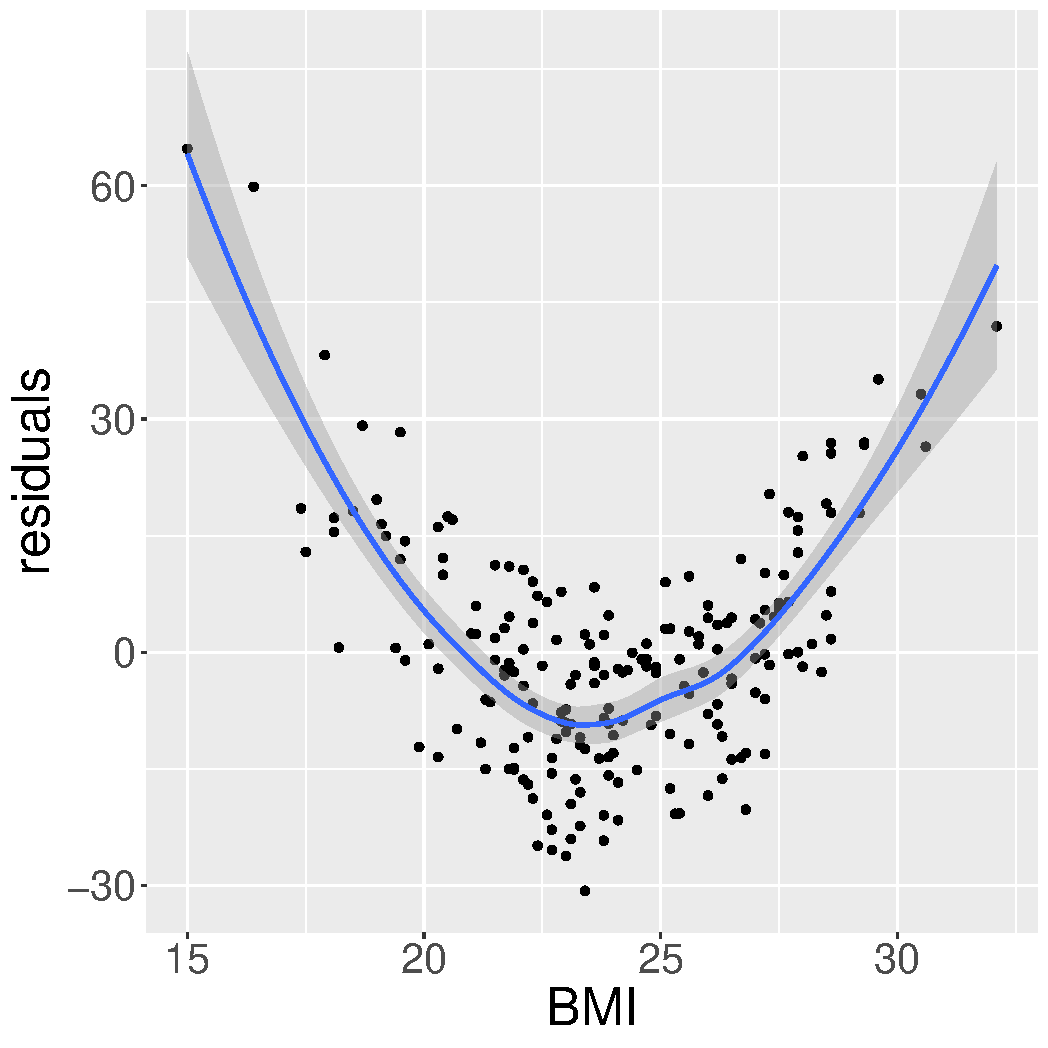
\includegraphics[width=0.7\textwidth]{./figures/A1-BMI.pdf}
\end{center} 

(similar plots can be automatically generated using the \texttt{crPlots} or
\texttt{ceresPlots} function from the car package). A p-value for testing the correct
specification of the functional form for the covariate can be obtained
using the \texttt{cumres} function from the gof package:
\lstset{language=r,label= ,caption= ,captionpos=b,numbers=none}
\begin{lstlisting}
cumres(e.lm, variable = "BMI")
\end{lstlisting}

\begin{verbatim}

    p-value(Sup) p-value(L2)
BMI            0           0

Based on 1000 realizations.
\end{verbatim}

\emph{Remedies}: if a trend is found, a possible remedy is to use splines to model the
non-linear relationship, e.g. 
\lstset{language=r,label= ,caption= ,captionpos=b,numbers=none}
\begin{lstlisting}
e.gam <- mgcv::gam(Y1 ~ Gender + Age + Gene + s(BMI), data = dfW)
\end{lstlisting}

In this simple example, it looks like a quadratic function of BMI
would be enough:
\lstset{language=r,label= ,caption= ,captionpos=b,numbers=none}
\begin{lstlisting}
e.lm.1 <- lm(Y1 ~ Gender + Age + Gene + BMI + I(BMI^2), data = dfW)
cumres(e.lm.1, variable = "BMI")
\end{lstlisting}

\begin{verbatim}

    p-value(Sup) p-value(L2)
BMI        0.268       0.444

Based on 1000 realizations.
\end{verbatim}
Note that this type of test is not appropriate to detect missing
interaction:
\lstset{language=r,label= ,caption= ,captionpos=b,numbers=none}
\begin{lstlisting}
cumres(e.lm.1, variable = "Age")
\end{lstlisting}

\begin{verbatim}

    p-value(Sup) p-value(L2)
Age        0.074       0.768

Based on 1000 realizations.
\end{verbatim}
while the display of the residuals can be informative
\lstset{language=r,label= ,caption= ,captionpos=b,numbers=none}
\begin{lstlisting}
gg <- ggplot(dfW, aes(x = Age, y = residuals(e.lm.1))) + geom_point() + geom_smooth()
gg
\end{lstlisting}


\begin{center}
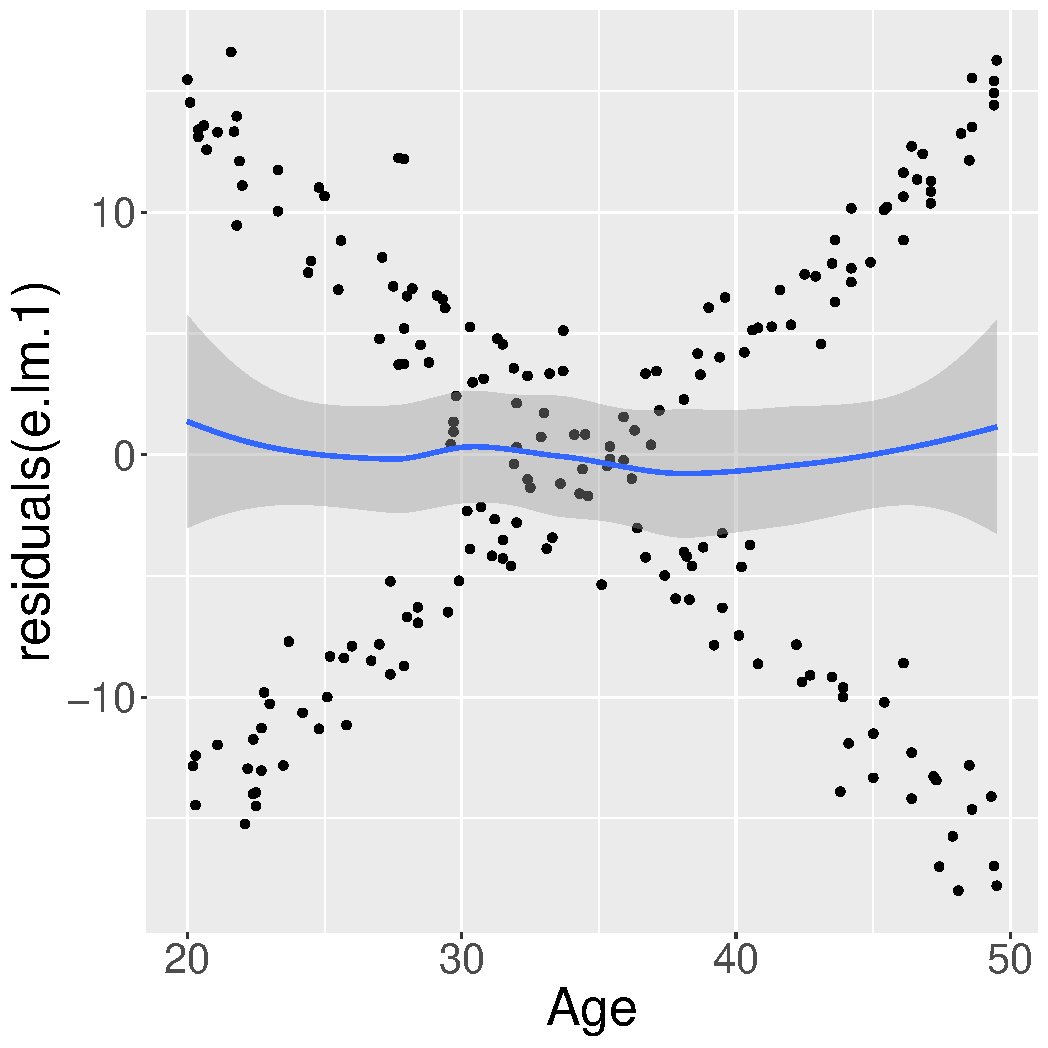
\includegraphics[width=0.8\textwidth]{./figures/A1-Age.pdf}
\end{center} 

\begin{itemize}
\item \textbf{checking for interactions} is hard because the number of possible
interactions grows quickly with the number of covariates. A typical
test would be to compare a model with interactions to a model
without interactions:
\end{itemize}
\lstset{language=r,label= ,caption= ,captionpos=b,numbers=none}
\begin{lstlisting}
e.lm.2 <- update(e.lm, Y1 ~ Gender*Age + Gene + BMI + I(BMI^2))
anova(e.lm.1, e.lm.2)
\end{lstlisting}

\begin{verbatim}
Analysis of Variance Table

Model 1: Y1 ~ Gender + Age + Gene + BMI + I(BMI^2)
Model 2: Y1 ~ Gender + Age + Gene + BMI + I(BMI^2) + Gender:Age
  Res.Df     RSS Df Sum of Sq      F    Pr(>F)    
1    193 16345.2                                  
2    192   509.8  1     15835 5963.5 < 2.2e-16 ***
---
Signif. codes:  0 ‘***’ 0.001 ‘**’ 0.01 ‘*’ 0.05 ‘.’ 0.1 ‘ ’ 1
\end{verbatim}
Note that in that case a test on the cumulative residuals process
would not detect any issue:
\lstset{language=r,label= ,caption= ,captionpos=b,numbers=none}
\begin{lstlisting}
cumres(e.lm.1, variable = "predicted")
\end{lstlisting}

\begin{verbatim}

          p-value(Sup) p-value(L2)
predicted        0.664       0.778

Based on 1000 realizations.
\end{verbatim}

\emph{Remedies}: this is a harder situation. When only few interactions are
considered, a possible strategy would be to include all of them and
perform backward selection. But then the p-values returned by \texttt{lm} for
the parameters related to the interactions (here \texttt{Gender}, \texttt{Age}, and
\texttt{Gender:Age}) will often be incorrect. Otherwise adding all possible
interactions and use a lasso/group-lasso penalty with post selection
inference. If the aim is prediction (and no inference), use more
flexible but less interpretable models (e.g. random forest).

\bigskip

\begin{itemize}
\item A last possible issue arise when the \textbf{outcome variable is not
studied on the right scale}. Consider the model using a square root
transformation:
\end{itemize}
\lstset{language=r,label= ,caption= ,captionpos=b,numbers=none}
\begin{lstlisting}
e.sqrt.lm <- lm(sqrt(Y1) ~ Gender*Age + Gene + BMI + I(BMI^2), data = dfW)
\end{lstlisting}

\clearpage

Diagnostic plots indicates lack of fit (first line, first plot) and
heteroschedasticity (second line first plot):
\lstset{language=r,label= ,caption= ,captionpos=b,numbers=none}
\begin{lstlisting}
autoplot(e.sqrt.lm)
\end{lstlisting}

\begin{center}
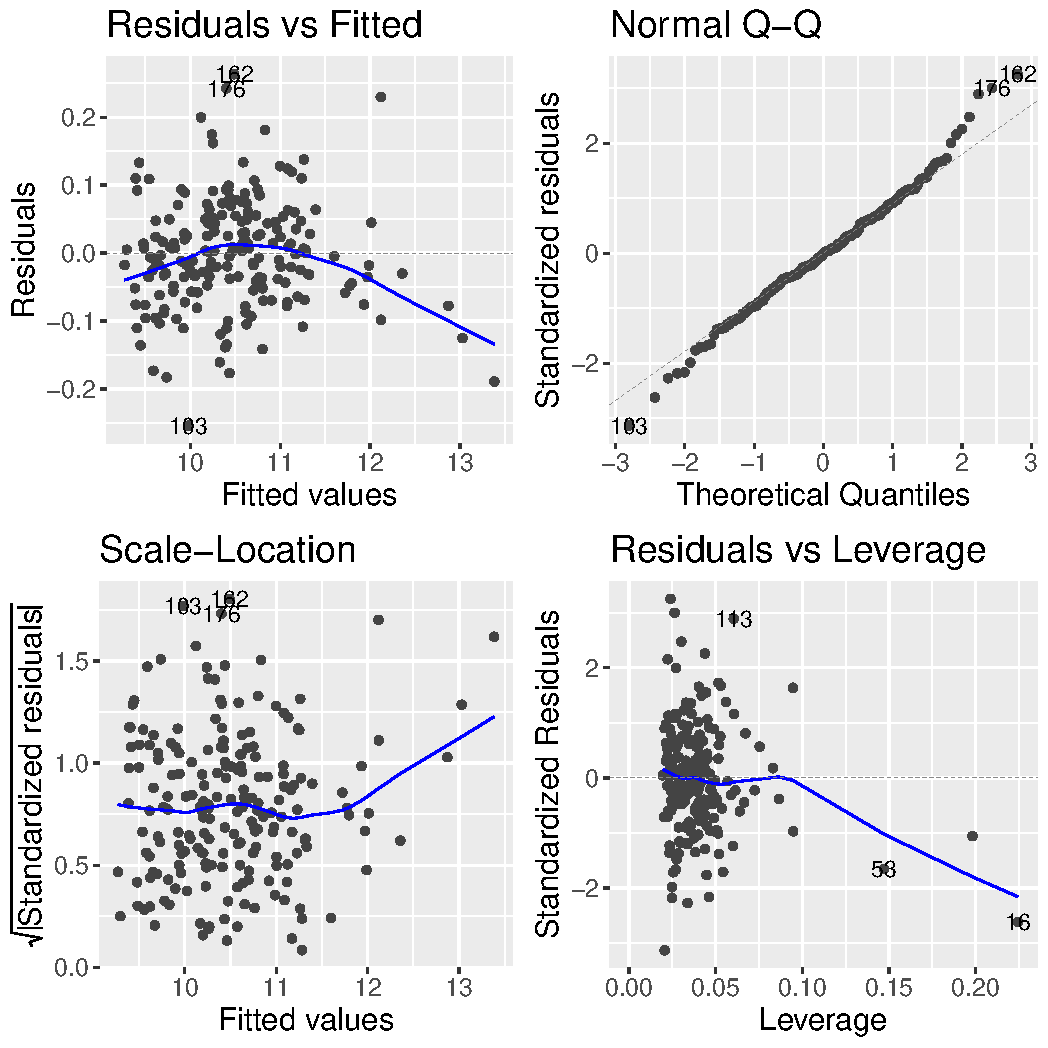
\includegraphics[width=0.8\textwidth]{./figures/A1-scale.pdf}
\end{center} 

We can use cumres and see that the link function seems inappropriate:
\lstset{language=r,label= ,caption= ,captionpos=b,numbers=none}
\begin{lstlisting}
cumres(e.sqrt.lm, variable = "predicted")
\end{lstlisting}

\begin{verbatim}

          p-value(Sup) p-value(L2)
predicted            0       0.001

Based on 1000 realizations.
\end{verbatim}

\clearpage

In that case a box-cox transformation can be useful as it suggests to
square the outcome:
\lstset{language=r,label= ,caption= ,captionpos=b,numbers=none}
\begin{lstlisting}
M <- MASS::boxcox(e.sqrt.lm, lambda = seq(-1,4,by=0.1))
M$x[which.max(M$y)]
\end{lstlisting}

\begin{verbatim}
[1] 1.828283
\end{verbatim}

Note that it seems to sometimes also suggest weird transformations:
\lstset{language=r,label= ,caption= ,captionpos=b,numbers=none}
\begin{lstlisting}
M <- MASS::boxcox(lm(log(Y1) ~ Gender*Age + Gene + BMI + I(BMI^2), data = dfW), lambda = seq(-10,10,by=0.1))
M$x[which.max(M$y)]
\end{lstlisting}

\begin{verbatim}
[1] 5.4
\end{verbatim}
(the results should be 0)

\subsubsection{\textbf{(A4)}: normal distribution}
\label{sec:org49be381}

\textbf{(A4)} can be tested using an histogram of the standardized residuals:
\lstset{language=r,label= ,caption= ,captionpos=b,numbers=none}
\begin{lstlisting}
hist(residuals(e.lm.2, type = "pearson"), freq = FALSE, breaks = 10)
curve(dnorm,-3,3,add =TRUE,col = "red")
\end{lstlisting}

\begin{center}
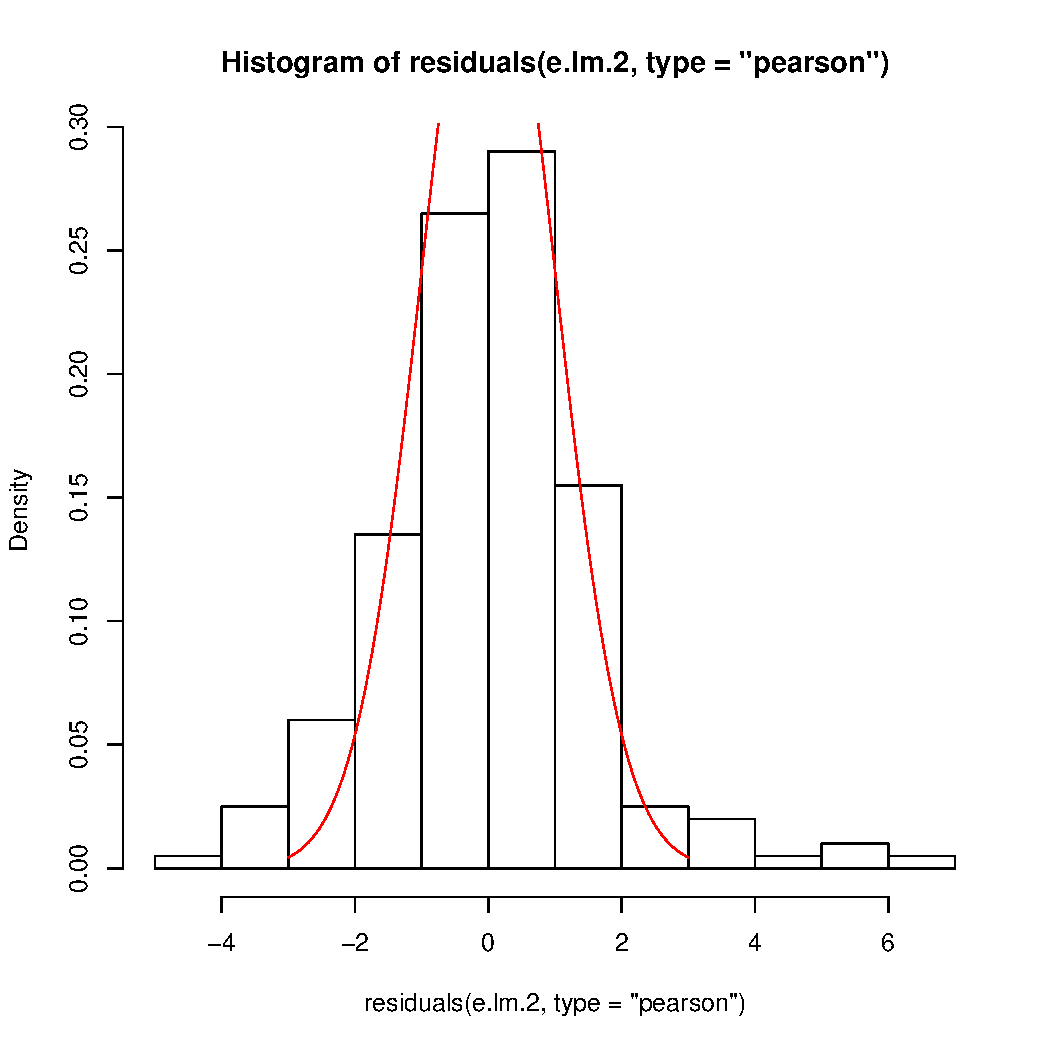
\includegraphics[width=0.8\textwidth]{./figures/A4-hist-res.pdf}
\end{center}

where the histogram should be close to the shape of the standard
normal distribution (red curve). We could reject \textbf{(A4)} but accept
\textbf{(A4-bis)} in the case where the distribution has heavy tails but is
still unimodal and symmetric. While intuitive, this method is
sensitive to the discretization of the residuals values (argument
break) and a qq-plot is often preferred:
\lstset{language=r,label= ,caption= ,captionpos=b,numbers=none}
\begin{lstlisting}
qqtest::qqtest(residuals(e.lm.2, type = "pearson"))
\end{lstlisting}

\begin{center}
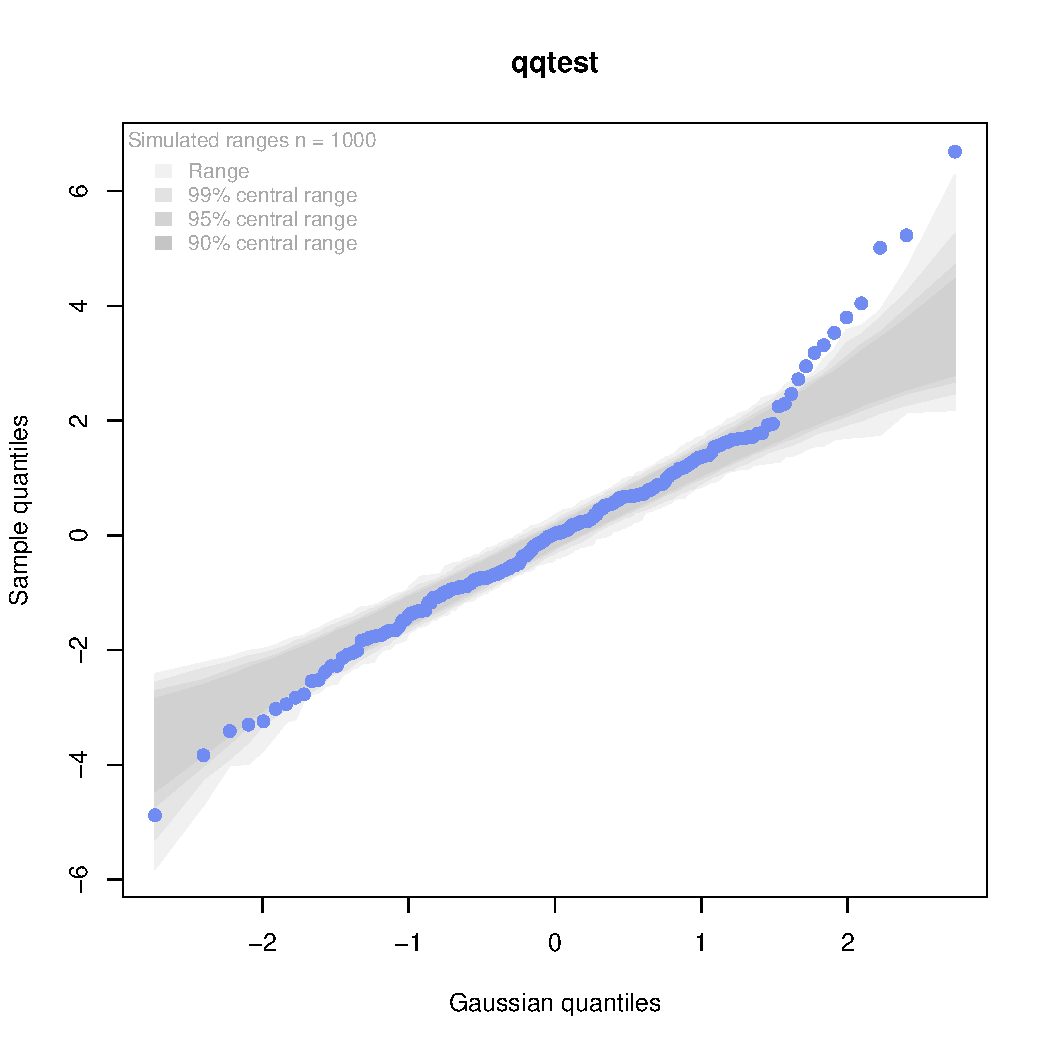
\includegraphics[width=0.8\textwidth]{./figures/A4-qqplot-res.pdf}
\end{center}

Here the points should follow a straight line and be within the shaded
area. We could reject \textbf{(A4)} but accept \textbf{(A4-bis)} in the case where
deviation to the straight line mostly arise in the tails.  Statistical
test (like a shapiro test) are not recommended since they do not
enable us to know whether we reject \textbf{(A4)} or \textbf{(A4bis)}. 

\bigskip

\emph{Remedies}: when \textbf{(A4)} is rejected but not \textbf{(A4-bis)}, the main
concern is about the validity of the traditional asymptotic
results. This is not critical in a linear regression where our
variance estimator is consistent and the central limit theorem ensures
asymptotic normality: instead of having exact p-values/CI they are
only asymptotically valid. If the sample size is not too small they
will hold; otherwise permutation test are a good alternative. In more
complex models, robust standard errors or non-parametric bootstrap can
be used for large enough samples to obtain p-values/CI robust to
deviation to the normal distribution. \newline A more serious problem
arises when \textbf{(A4-bis)} is rejected. In that case one should consider
whether the expected outcome is really relevant. Alternative
approaches include transformation of the outcome or use of alternative
regression models (quantile regression, probability index models,
finite mixture models).

\bigskip

Note 1: the \texttt{type} argument indicates the type of residuals we want to
extract. Raw residuals are \(\hat{\varepsilon} = Y-\hat{Y}\), i.e. the
observed minus the fitted values. In models more complex than a
univariate linear regression, the raw residuals may not be iid. This
makes it difficult to assess the validity of the assumptions. In such
cases we display instead diagnostics for normalized residuals that, if
the assumptions of the model are correct, should follow a standard
normal distribution.

\bigskip

Note 2: an alternative to the \texttt{qqtest} function is the \texttt{qqPlot}
function from the car package.

\subsubsection{\textbf{(A2)}: Homeschedasticity}
\label{sec:orgbeedb2d}
Homoschedasticity can be inspected by displaying the residuals along
the fitted values:
\lstset{language=r,label= ,caption= ,captionpos=b,numbers=none}
\begin{lstlisting}
d$residuals <- residuals(e.lm.2, type = "pearson")
d$fitted <- fitted(e.lm.2)
gg <- ggplot(d, aes(x = fitted)) + ylab("residuals")
gg <- gg + geom_smooth(aes(y = residuals^2-1))
gg <- gg + geom_point(aes(y = residuals))
gg
\end{lstlisting}


\begin{center}
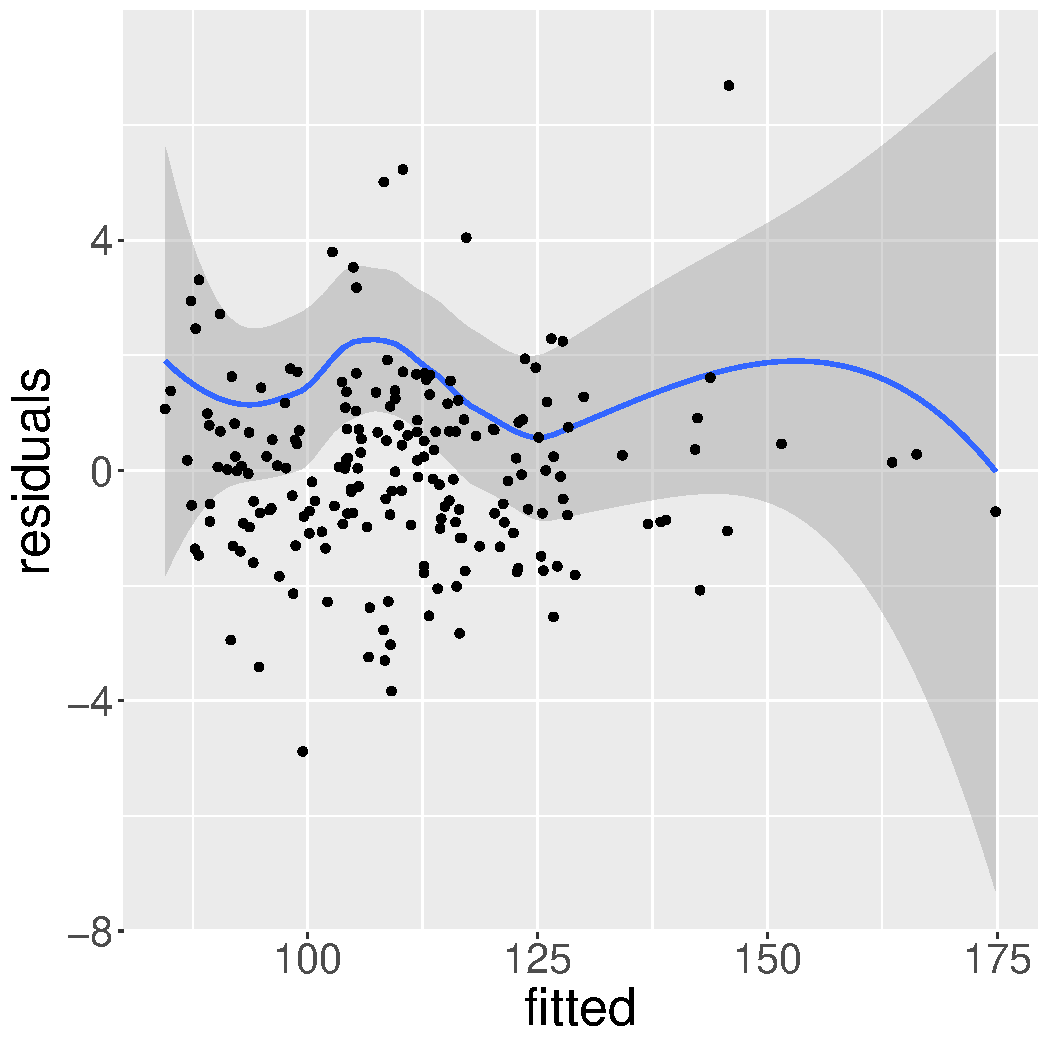
\includegraphics[width=0.8\textwidth]{./figures/A2-smooth.pdf}
\end{center}

(see also the function \texttt{spreadLevelPlot} from the car package). It is
also possible to have a global statistical test (Breusch-Pagan test):
\lstset{language=r,label= ,caption= ,captionpos=b,numbers=none}
\begin{lstlisting}
ncvTest(e.lm.2)
\end{lstlisting}

\begin{verbatim}
Non-constant Variance Score Test 
Variance formula: ~ fitted.values 
Chisquare = 0.2765166, Df = 1, p = 0.59899
\end{verbatim}

Alternatively one can look along a specific regressor:
\lstset{language=r,label= ,caption= ,captionpos=b,numbers=none}
\begin{lstlisting}
gg <- ggplot(d, aes(x = Gender, y = residuals)) + ylab("residuals")
gg <- gg + geom_boxplot()
gg
\end{lstlisting}

\begin{center}
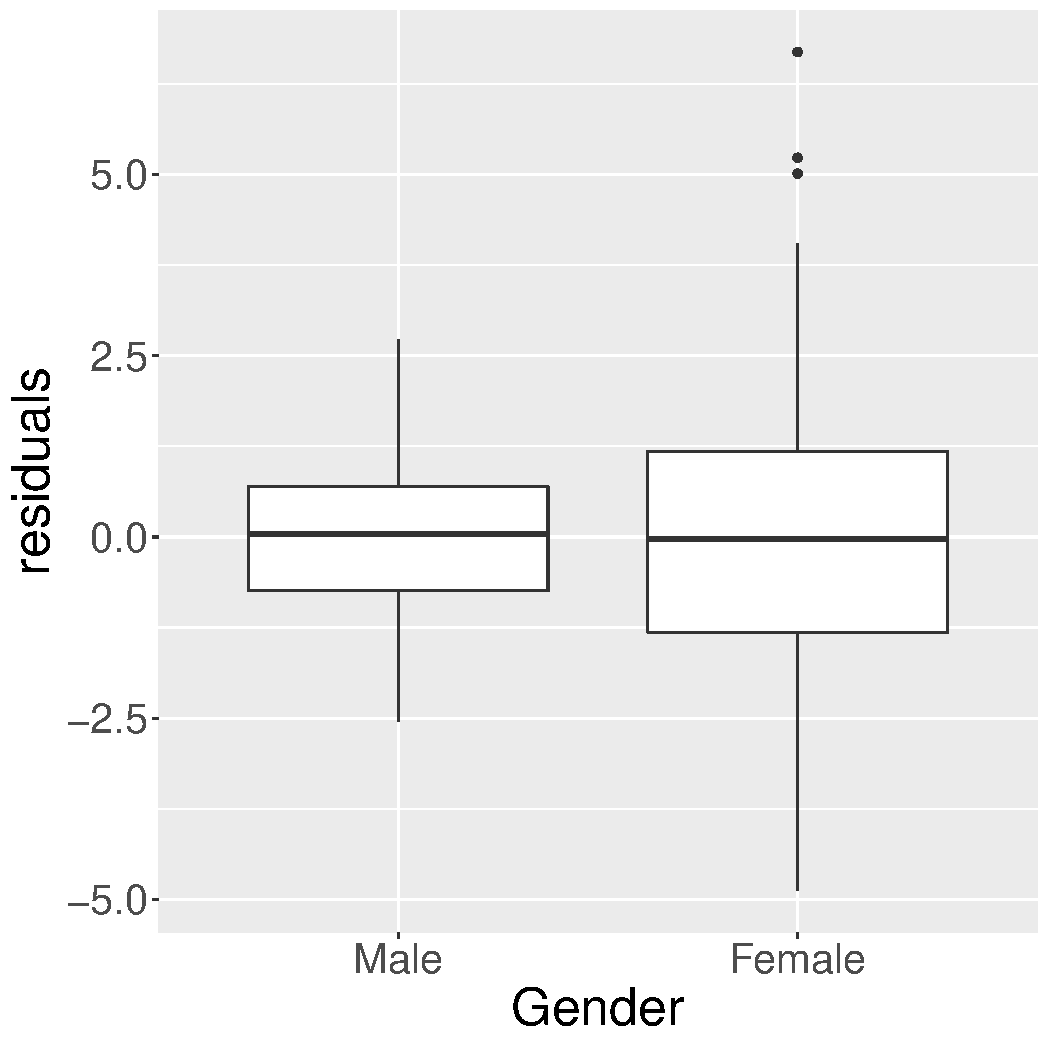
\includegraphics[width=0.8\textwidth]{./figures/A2-boxplot.pdf}
\end{center}

or investigate look how the squared residuals relates to the
regressors:
\lstset{language=r,label= ,caption= ,captionpos=b,numbers=none}
\begin{lstlisting}
summary(lm(residuals(e.lm.2)^2 ~ Gender + Age + Gene + BMI, data = dfW))$coef
\end{lstlisting}

\begin{verbatim}
               Estimate Std. Error    t value     Pr(>|t|)
(Intercept)  3.27861402 3.07851696  1.0649979 2.882006e-01
GenderMale  -2.92345176 0.69766213 -4.1903546 4.227552e-05
Age         -0.03880792 0.03964689 -0.9788388 3.288787e-01
GeneB        0.41620970 0.87214618  0.4772247 6.337393e-01
GeneC        0.18989247 0.82390876  0.2304775 8.179636e-01
BMI          0.07868374 0.11627415  0.6767088 4.993968e-01
\end{verbatim}

\emph{Remedies}: in presence of global heteroschadasticity (first graph),
transforming the outcome can be a solution. Otherwise one should
reflect about possible source of heteroschadasticity (e.g. correlated
observations, mixture of populations) and model them. When the
heteroschadasticity is related to a single variable, one can for
instance use the \texttt{gls} function to model this variance:

\clearpage

\lstset{language=r,label= ,caption= ,captionpos=b,numbers=none}
\begin{lstlisting}
e.gls <- gls(Y1 ~ Gender + Age + Gene + BMI + I(BMI^2) + Gender:Age, 
	     data = dfW,
	     weight = varIdent(form=~1|Gender))
summary(e.gls$modelStruct)
\end{lstlisting}

\begin{verbatim}
Variance function:
 Structure: Different standard deviations per stratum
 Formula: ~1 | Gender 
 Parameter estimates:
    Male   Female 
1.000000 2.096499
\end{verbatim}

\lstset{language=r,label= ,caption= ,captionpos=b,numbers=none}
\begin{lstlisting}
summary(
    lm(residuals(e.gls, type = "normalized")^2 ~ Gender + Age + Gene + BMI, data = dfW)
)$coef
\end{lstlisting}

\begin{verbatim}
               Estimate Std. Error    t value  Pr(>|t|)
(Intercept)  0.95513614 0.92435359  1.0333017 0.3027491
GenderMale   0.01093174 0.20947960  0.0521852 0.9584348
Age         -0.01802386 0.01190435 -1.5140566 0.1316390
GeneB        0.10417273 0.26187007  0.3978031 0.6912127
GeneC       -0.05737372 0.24738633 -0.2319195 0.8168450
BMI          0.02549938 0.03491241  0.7303817 0.4660380
\end{verbatim}


\subsubsection{\textbf{(A5)}: Influential observations}
\label{sec:org988ae93}

The \texttt{influence} method can be used to output what is the impact of
each observation on each estimated parameter:
\lstset{language=r,label= ,caption= ,captionpos=b,numbers=none}
\begin{lstlisting}
if.lme <- influence(e.lm.2)
if.lme$coefficient[1:6,1:4]
\end{lstlisting}

\begin{verbatim}
    (Intercept)    GenderMale           Age         GeneB
1 -0.0768500758 -1.729088e-02 -8.430716e-06 -6.556256e-03
2  0.0033441763  8.848004e-04 -1.583090e-06 -1.330066e-03
3 -1.4634794147 -8.233340e-02 -2.155624e-04  4.249566e-02
4  0.0759756521 -4.035183e-03  4.852756e-05 -8.238371e-04
5 -0.0427789759 -1.599394e-03  2.073558e-05 -8.720082e-03
6  0.0008298817  4.867202e-05  2.398257e-07 -3.293940e-06
\end{verbatim}

Here the value in the first line and third column indicates by how
much is changed the Age effect when removing the first observation.
\lstset{language=r,label= ,caption= ,captionpos=b,numbers=none}
\begin{lstlisting}
coef(update(e.lm.2, data = dfW[-1,]))-coef(e.lm.2)
\end{lstlisting}

\begin{verbatim}
 (Intercept)     GenderMale            Age          GeneB          GeneC            BMI 
7.685008e-02   1.729088e-02   8.430716e-06   6.556256e-03   8.024692e-03  -7.151957e-03 
    I(BMI^2) GenderMale:Age 
1.540482e-04  -6.600643e-04
\end{verbatim}

Large values (positive or negative) indicate influential
observations. The following plot displaying in red the coefficient
value and in black the influence of each individual can be useful:
\lstset{language=r,label= ,caption= ,captionpos=b,numbers=none}
\begin{lstlisting}
df1.gg <- data.frame(id = "true", as.data.frame(t(coef(e.lm.2))))
df2.gg <- data.frame(id = as.character(1:NROW(d)), 
		     sweep(if.lme$coefficient, FUN = "+", MARGIN = 2, STATS = coef(e.lm.2)))
dfL1.gg <- reshape2::melt(df1.gg, id.vars = "id")
dfL2.gg <- reshape2::melt(df2.gg, id.vars = "id")
gg.inf <-  ggplot() + facet_wrap(~variable, scales = "free", nrow = 2)
gg.inf <- gg.inf + geom_boxplot(data = dfL2.gg, aes(y = value))
gg.inf <- gg.inf + geom_hline(data = dfL1.gg, aes(yintercept = value), color = "red")
gg.inf
\end{lstlisting}

\begin{center}
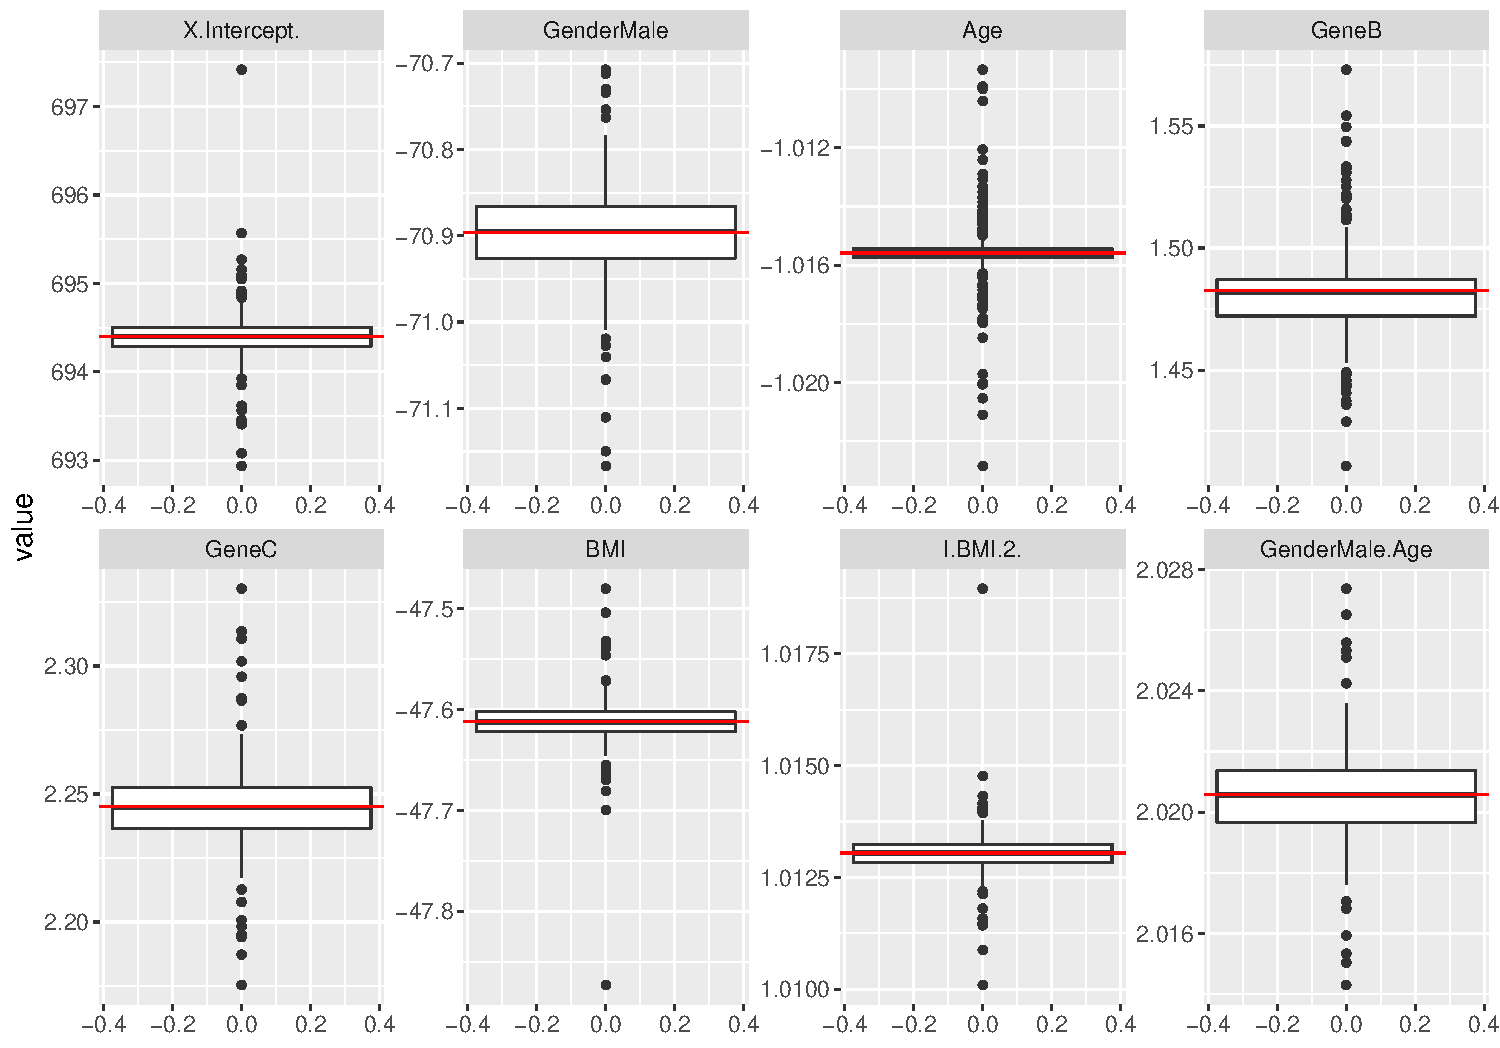
\includegraphics[width=\textwidth]{./figures/A5-boxplot.pdf}
\end{center}

When the aim is to perform prediction, global influence metrics such
as Cook's distance can be useful:
\lstset{language=r,label= ,caption= ,captionpos=b,numbers=none}
\begin{lstlisting}
autoplot(e.lm.2, which = 4)
\end{lstlisting}

\begin{center}
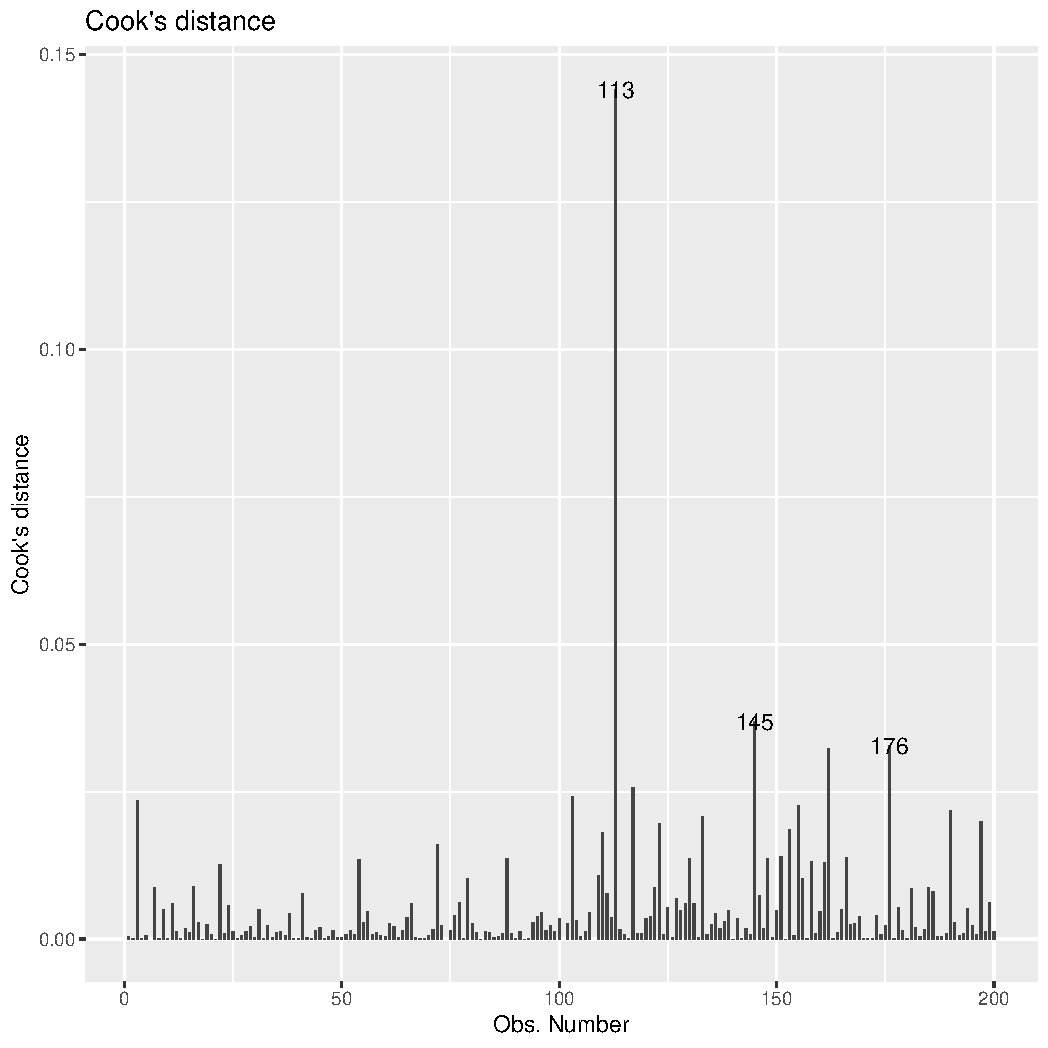
\includegraphics[width=0.8\textwidth]{./figures/A5-cook.pdf}
\end{center}


\subsubsection{Others [not recommanded unless specific reasons]}
\label{sec:org970337f}
Some people recommand to check the correlation between the explanatory
variables, with the argument that when very correlated it is difficult
to disantangle effects and thus to interpret the regression
coefficients. The VIF (variance inflation factor) is typically
recommanded to check that with values higher than 5 considered as
high:

\lstset{language=r,label= ,caption= ,captionpos=b,numbers=none}
\begin{lstlisting}
car::vif(e.lm.2)
\end{lstlisting}

\begin{verbatim}
                 GVIF Df GVIF^(1/(2*Df))
Gender      16.405278  1        4.050343
Age          2.107105  1        1.451587
Gene         1.070289  2        1.017127
BMI        153.493940  1       12.389267
I(BMI^2)   153.046502  1       12.371196
Gender:Age  17.937937  1        4.235320
\end{verbatim}

I personnally don't recommand this as an automatic check since in many
  settings co-linearity can be better assessed from the meaning of the
  variables than from a statistical test. It is also quite unclear to
  me why 5 is a good cut-off and we see in this example that we get
  values close to five (or higher) even though there is no issue.

\clearpage


\section{Partial residuals}
\label{sec:pRes}
\subsection{With respect to one variable}
\label{sec:orgac77490}

The partial residuals with respect to age are defined by removing the
effect of all the covariates but age on the outcome:
\begin{align*}
\hat{\varepsilon}^{Age}_i &= Y_i - \left(\alpha + \beta_{Gender} \Ind[Gender_i="Male"] + \beta_{GeneB} \Ind[Gene_i="B"] + \beta_{GeneC} \Ind[Gene_i="C"]  + \beta_{BMI} BMI_i\right)
\end{align*}
Using the following model coefficients:
\lstset{language=r,label= ,caption= ,captionpos=b,numbers=none}
\begin{lstlisting}
coef(e.lm)
\end{lstlisting}

\begin{verbatim}
(Intercept)  GenderMale         Age       GeneB       GeneC         BMI 
 91.5609817   3.7984283  -0.1358252   7.8328783   5.8120279   0.7364696
\end{verbatim}

and considering the first individual:
\lstset{language=r,label= ,caption= ,captionpos=b,numbers=none}
\begin{lstlisting}
d[1,]
\end{lstlisting}

\begin{verbatim}
  Id  Age Gender  BMI Gene    Y1    Y2       Y3 residuals   fitted
1  1 44.2   Male 23.8    A 109.1 120.8 131.7429 0.5188666 108.5811
\end{verbatim}

the partial residual relative to age is:
\begin{align*}
\hat{\varepsilon}^{Age}_1 &= 109.1 - \left(91.5610 + 3.7984 * 1 + 7.8329 * 0 + 5.8120 * 0 + 0.7365 * 23.8 \right) \\
                         &= 109.1 - 112.8881 = -3.7881
\end{align*}
At the dataset level, this type of partial residual is centered around
the expected value of the covariate times its effect (here
\(-0.1358252*34.4855 \approx -4.684\)). These partial residuals can be
computed using the \texttt{partialResidual} function from the butils package:
\lstset{language=r,label= ,caption= ,captionpos=b,numbers=none}
\begin{lstlisting}
pRes.noI <- partialResiduals(e.lm, var = "Age", keep.intercept = FALSE)
head(pRes.noI)
\end{lstlisting}

\begin{verbatim}
   Id  Age Gender  BMI Gene    Y1    Y2       Y3     pFit ranef  pResiduals
1:  1 44.2   Male 23.8    A 109.1 120.8 131.7429 112.8874     0  -3.7873855
2:  2 41.3   Male 27.5    B 123.2 133.9 136.3850 123.4452     0  -0.2452012
3:  3 27.4   Male 30.6    A 140.6 154.0 136.1408 117.8954     0  22.7046216
4:  4 35.3   Male 25.2    C 104.4 116.2 125.0175 119.7305     0 -15.3304708
5:  5 37.1   Male 21.8    A 105.0 113.2 123.6257 111.4144     0  -6.4144463
6:  6 29.9   Male 18.1    C 125.9 136.2 131.7966 114.5015     0  11.3984631
\end{verbatim}

or manually:
\lstset{language=r,label= ,caption= ,captionpos=b,numbers=none}
\begin{lstlisting}
keep.coef <- c("(Intercept)","GenderMale","GeneB","GeneC","BMI")
dfW$Y1[1] - model.matrix(e.lm)[1,keep.coef] %*% coef(e.lm)[keep.coef]
\end{lstlisting}

\begin{verbatim}
          [,1]
[1,] -3.787385
\end{verbatim}

A graphical display can be obtained using the \texttt{autoplot} function
(require the ggplot2 package):
\lstset{language=r,label= ,caption= ,captionpos=b,numbers=none}
\begin{lstlisting}
gg <- autoplot(pRes.noI)
\end{lstlisting}

\begin{center}
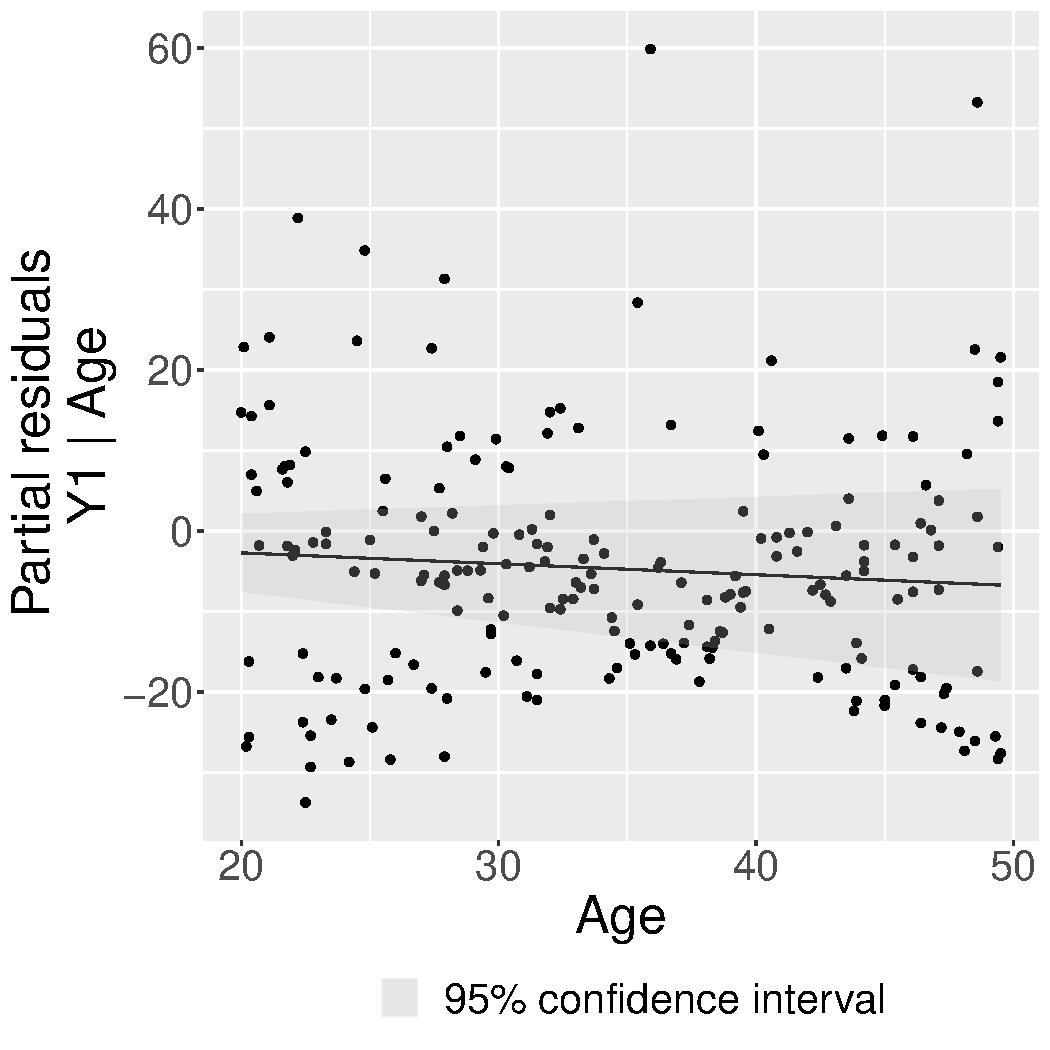
\includegraphics[width=0.7\textwidth]{./figures/fig-butils-plotConf-noI.pdf}
\end{center}

\begin{itemize}
\item An alternative definition do not remove the intercept effect:
\end{itemize}
\begin{align*}
\hat{\varepsilon}^{Age,\alpha}_i &= Y_i - \left(\beta_{Gender} \Ind[Gender_i="Male"] + \beta_{GeneB} \Ind[Gene_i="B"] + \beta_{GeneC} \Ind[Gene_i="C"] + \beta_{BMI} BMI_i \right)
\end{align*}
so now the residuals are centered around the intercept plus the
expected value of age times the age effect (here approximately 0). 

\clearpage

As before the partial residuals can either be obtained via the
\texttt{partialResiduals} function:
\lstset{language=r,label= ,caption= ,captionpos=b,numbers=none}
\begin{lstlisting}
pRes.I <- partialResiduals(e.lm, var = "Age", keep.intercept = TRUE)
head(pRes.I)
\end{lstlisting}

\begin{verbatim}
   Id  Age Gender  BMI Gene    Y1    Y2       Y3     pFit ranef pResiduals
1:  1 44.2   Male 23.8    A 109.1 120.8 131.7429 21.32640     0   87.77360
2:  2 41.3   Male 27.5    B 123.2 133.9 136.3850 31.88422     0   91.31578
3:  3 27.4   Male 30.6    A 140.6 154.0 136.1408 26.33440     0  114.26560
4:  4 35.3   Male 25.2    C 104.4 116.2 125.0175 28.16949     0   76.23051
5:  5 37.1   Male 21.8    A 105.0 113.2 123.6257 19.85346     0   85.14654
6:  6 29.9   Male 18.1    C 125.9 136.2 131.7966 22.94056     0  102.95944
\end{verbatim}

or manually: 
\lstset{language=r,label= ,caption= ,captionpos=b,numbers=none}
\begin{lstlisting}
keep.coef <- c("GenderMale","GeneB","GeneC","BMI")
dfW$Y1[1] - model.matrix(e.lm)[1,keep.coef] %*% coef(e.lm)[keep.coef]
\end{lstlisting}

\begin{verbatim}
        [,1]
[1,] 87.7736
\end{verbatim}

This corresponds to what the \texttt{plotConf} function is displaying (R
package lava available on CRAN):
\lstset{language=r,label= ,caption= ,captionpos=b,numbers=none}
\begin{lstlisting}
lava::plotConf(e.lm, var1 = "Age")
\end{lstlisting}

\begin{center}
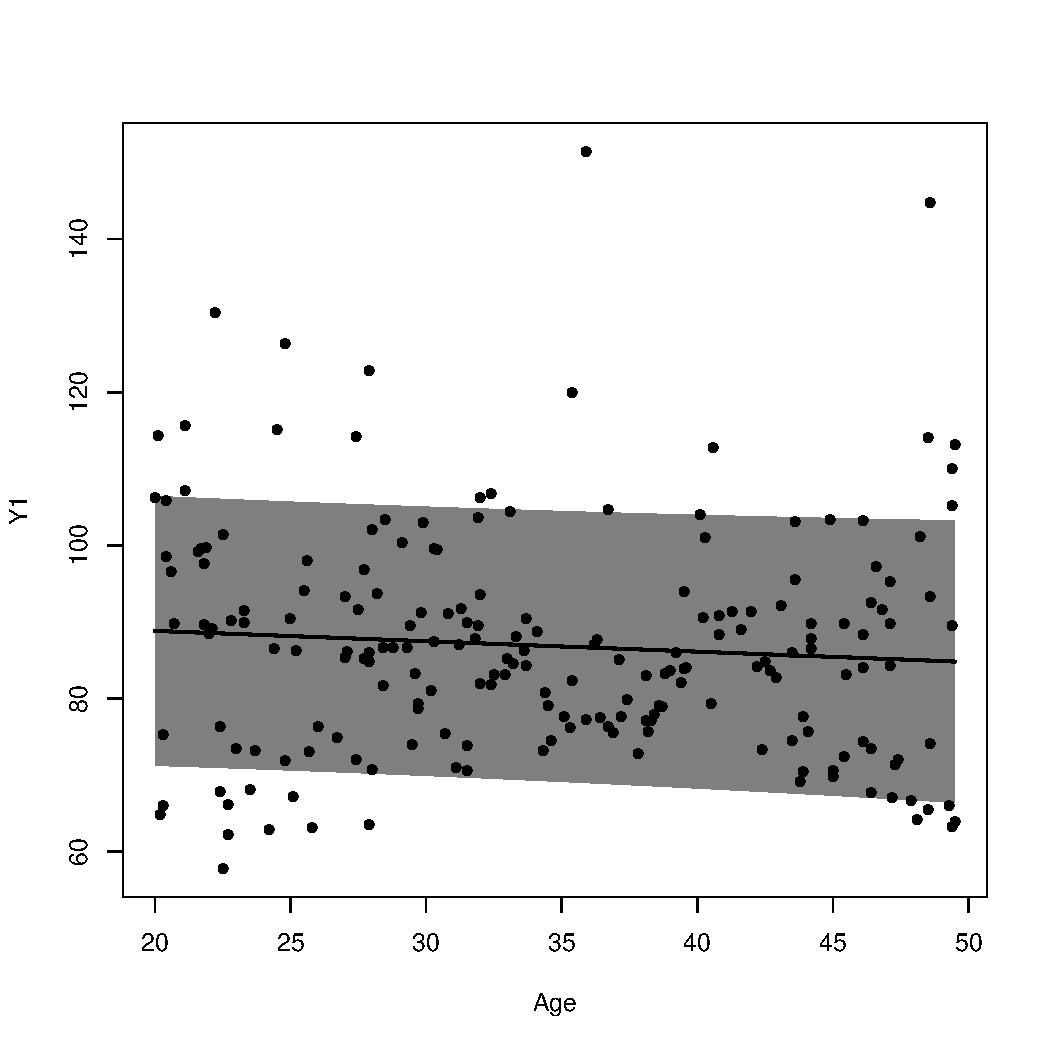
\includegraphics[width=0.7\textwidth]{./figures/fig-lava-plotConf.pdf}
\end{center}

Note that it is also possible to display the partial residuals for a
categorical variable:
\lstset{language=r,label= ,caption= ,captionpos=b,numbers=none}
\begin{lstlisting}
pRes.cat <- partialResiduals(e.lm, var = "Gene", keep.intercept = TRUE)
gg <- autoplot(pRes.cat)
gg
\end{lstlisting}


\begin{center}
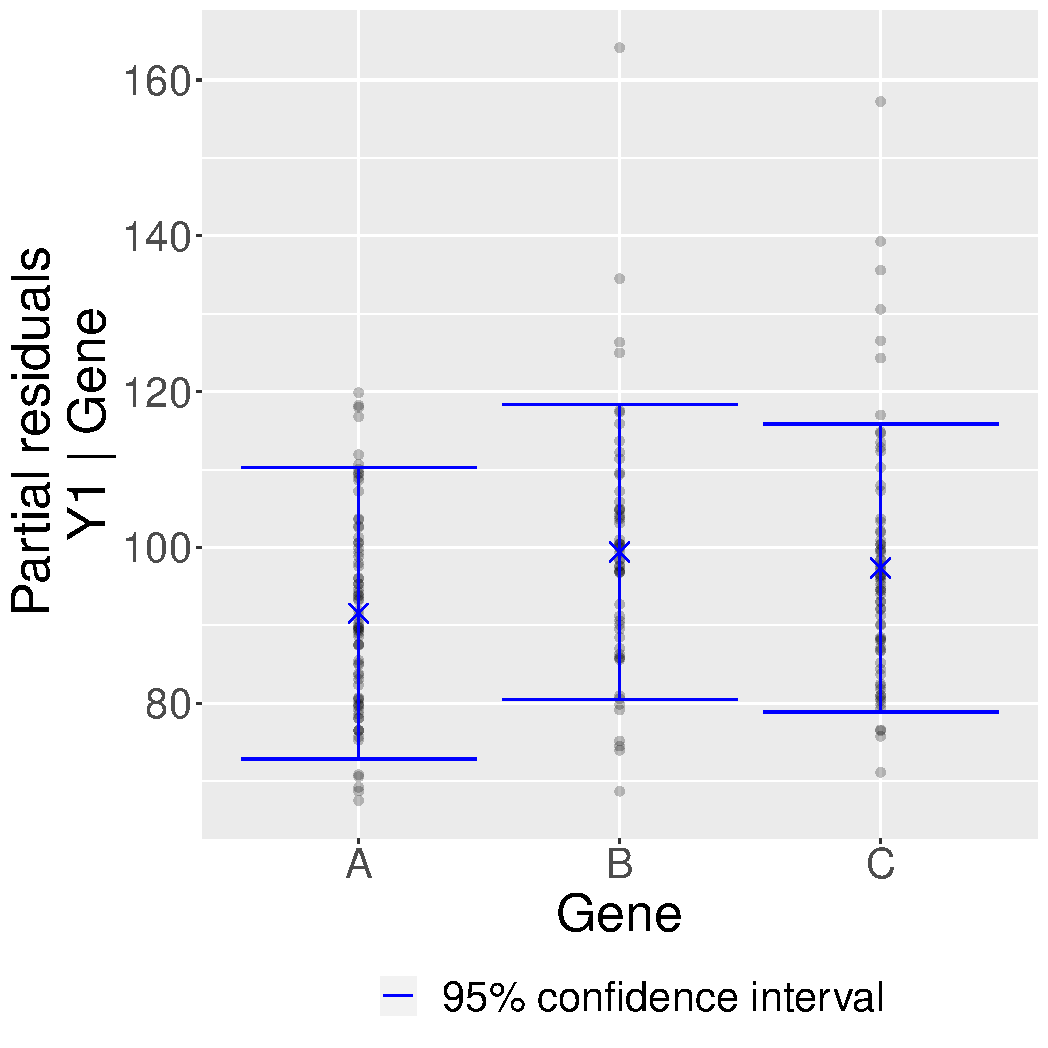
\includegraphics[width=0.7\textwidth]{./figures/fig-butils-plotConf-categorical.pdf}
\end{center}

\subsection{With respect to an interaction between two variables (one continuous, one categorical)}
\label{sec:org9a6e7c2}

Consider now a model where the age effect can be different for males
and females:
\lstset{language=r,label= ,caption= ,captionpos=b,numbers=none}
\begin{lstlisting}
e.lmI <- lm(Y1 ~ Gender * Age + Gene + BMI, data = dfW)
\end{lstlisting}

The partial residuals can be defined in a similar way as before. Here
the effect of Age and Gender (and their interaction) are not
substracted from the outcome:
\lstset{language=r,label= ,caption= ,captionpos=b,numbers=none}
\begin{lstlisting}
gg <- autoplot(partialResiduals(e.lmI, var = c("Age","Gender")))
\end{lstlisting}

\begin{center}
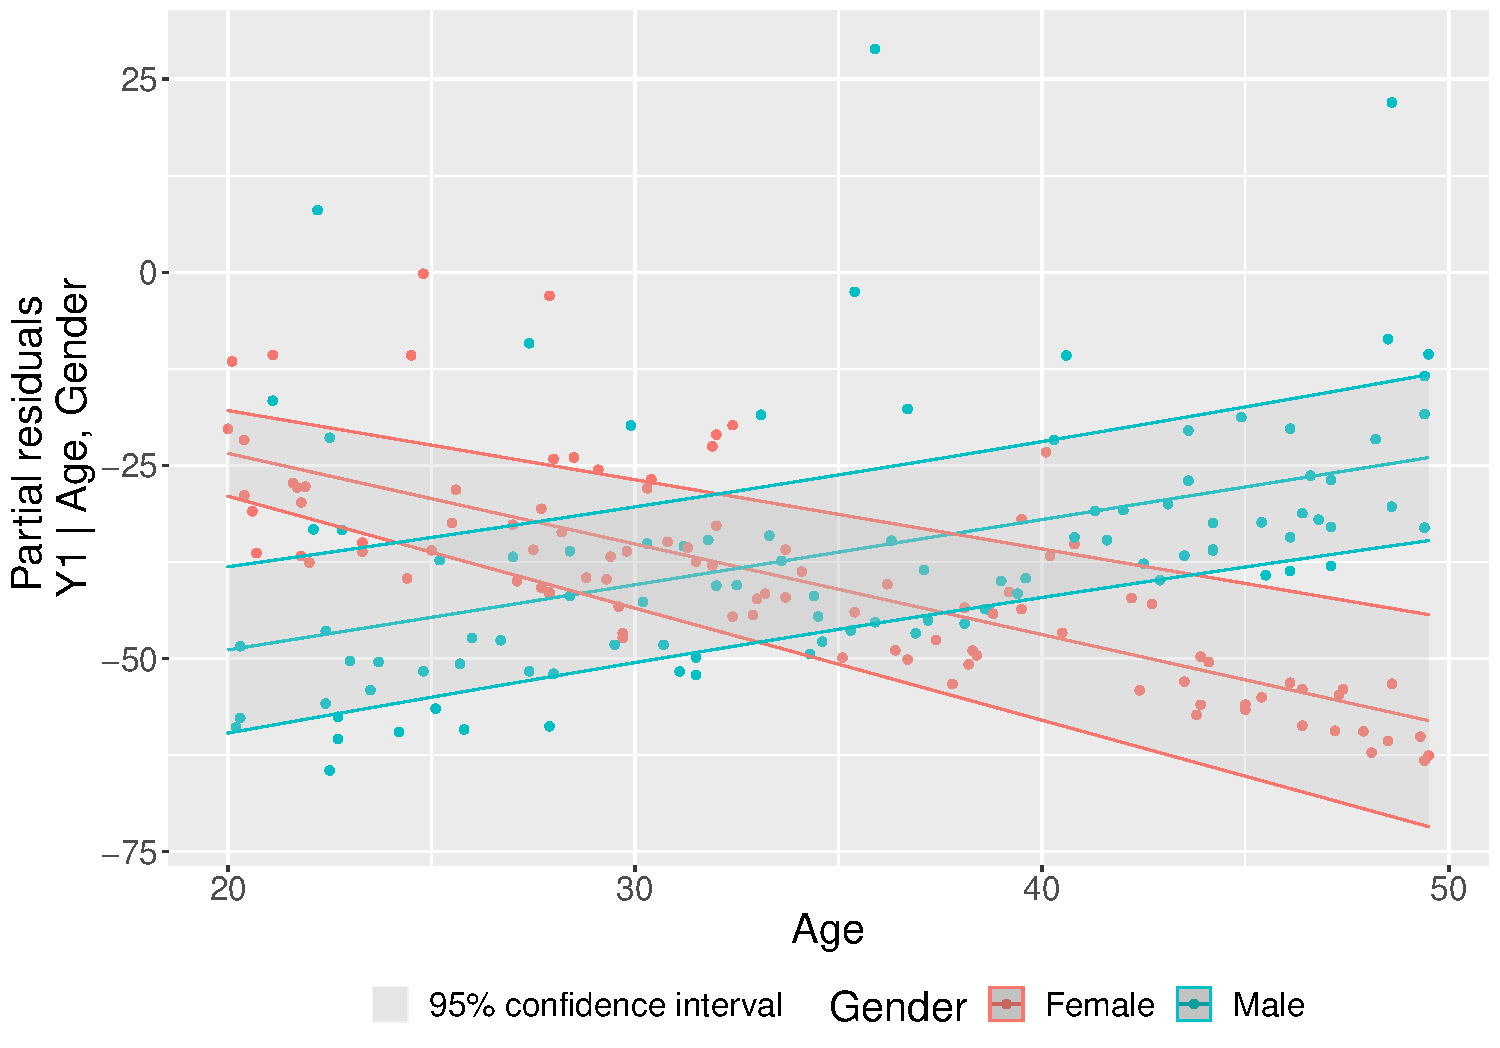
\includegraphics[width=0.7\textwidth]{./figures/fig-butils-plotConf-interaction.pdf}
\end{center}

\subsection{Customizing a partial residual plot}
\label{sec:org24a45c5}

The autoplot function returns the ggplot object:
\lstset{language=r,label= ,caption= ,captionpos=b,numbers=none}
\begin{lstlisting}
gg <- autoplot(partialResiduals(e.lm, var = "Gene", keep.intercept = TRUE))
class(gg)
\end{lstlisting}

\begin{verbatim}
[1] "gg"     "ggplot"
\end{verbatim}

So it can be easily customized, e.g. the text can be made bigger by
doing:
\lstset{language=r,label= ,caption= ,captionpos=b,numbers=none}
\begin{lstlisting}
gg + theme(text = element_text(size=25))
\end{lstlisting}
\end{document}